% =========================================================================
% DRAFT: experience-report framing.  Uses \documentclass{article} for local
% compilation.  For POPL 2027 submission switch to:
%   \documentclass[acmsmall,review,anonymous]{acmart}
% with the ACM CCS/keywords block below uncommented.
%
% ACM metadata for final submission:
%   \acmJournal{PACMPL} \acmVolume{0} \acmNumber{POPL}
%   \acmYear{2027} \acmMonth{1} \setcopyright{none}
%
% CCS:
%   Theory of computation~Proof theory        [500]
%   Theory of computation~Logic and verification [300]
%   Theory of computation~Type theory         [300]
%
% Keywords: flag algebras, Lean 4, proof by reflection, semidefinite
%   programming, Turan density, interactive theorem proving,
%   tactic metaprogramming, extremal combinatorics, experience report
% =========================================================================
\documentclass{article}

\usepackage{hyperref}
\usepackage{amsmath}
\usepackage{mathtools}
\usepackage{amssymb}
\usepackage{amsthm}
\usepackage{dsfont}
\usepackage{stmaryrd}
\usepackage{xcolor}
\usepackage{listings}
\usepackage{booktabs}
\usepackage{microtype}
\usepackage{fullpage}
\usepackage{authblk}
\usepackage{cleveref}
\usepackage{tikz}

% ---- Theorem environments -----------------------------------------------
\newtheorem{theorem}{Theorem}[section]
\newtheorem{lemma}[theorem]{Lemma}
\newtheorem{definition}[theorem]{Definition}
\newtheorem{example}[theorem]{Example}
\newtheorem{remark}[theorem]{Remark}

% ---- Macros -------------------------------------------------------------
\newcommand{\R}{\mathbb{R}}
\newcommand{\Q}{\mathbb{Q}}
\newcommand{\N}{\mathbb{N}}
\newcommand{\Fin}[1]{\mathsf{Fin}(#1)}
\newcommand{\Flag}[1]{\mathcal{F}^{#1}}
\newcommand{\FlagAlg}[1]{\mathcal{A}^{#1}}
\newcommand{\poshom}[1]{\Phi^{#1}}
\newcommand{\den}[2]{p(#1,\,#2)}
\newcommand{\tdensity}[2]{\pi(#1;\,#2)}
\newcommand{\forbLE}[1]{\leq_{\operatorname{Forb}(#1)}}
\newcommand{\forbLES}[2]{\leq_{#1,\operatorname{Forb}(#2)}}
\newcommand{\lean}[1]{\texttt{#1}}

\tikzset{
  graph vertex/.style={circle, draw, fill=white, inner sep=0pt, minimum size=4.5pt},
  graph root/.style={circle, draw, fill=black, inner sep=0pt, minimum size=4.5pt},
  graph edge/.style={line width=0.45pt}
}

% Lean code style
\lstdefinelanguage{Lean4}{
  keywords={def,theorem,lemma,instance,structure,class,import,open,namespace,
             end,where,fun,let,have,show,by,match,with,if,then,else,
             return,do,for,in,noncomputable,abbrev,variable,section,
             native_decide,decide,norm_num,simp,ring,linarith,omega,
             exact,apply,rw,calc,intro,constructor,use,refine,obtain,
             rcases,cases,induction,assumption,contradiction,trivial,rfl,
             macro,elab},
  keywordstyle=\color{blue!70!black}\bfseries,
  comment=[l]{--},
  commentstyle=\color{gray}\itshape,
  stringstyle=\color{orange!80!black},
  morestring=[b]",
  sensitive=true,
  basicstyle=\ttfamily\small,
  breaklines=true,
  columns=fullflexible,
  escapeinside={(*@}{@*)},
  literate=
    {->}{{$\to$}}2
    {<-}{{$\leftarrow$}}2
    {<=}{{$\leq$}}1
    {>=}{{$\geq$}}1
    {alpha}{{$\alpha$}}1
    {forall}{{$\forall$}}1
    {exists}{{$\exists$}}1
    {phi}{{$\phi$}}1
    {psi}{{$\psi$}}1
}
\lstset{language=Lean4, frame=single, framesep=4pt,
        rulecolor=\color{black!20}, backgroundcolor=\color{gray!5}}

% =========================================================================
\title{A Verified Flag Algebra Pipeline in Lean~4: \\
       An Experience Report}
\date{}

\author[1]{Gyeongwon Jeong}
\author[1]{Seonghun Park}
\author[1]{Jihoon Hyun}
\author[2]{Sang-il Oum}
\author[3]{Hongseok Yang}
\affil[1]{School of Computing, KAIST, South Korea}
\affil[2]{Discrete Mathematics Group, Institute for Basic Science (IBS), South Korea}
\affil[3]{School of Computational Sciences, Korea Institute for Advanced Study (KIAS), South Korea}

% =========================================================================
\begin{document}
\maketitle

\begin{abstract}
Flag algebras are a proof method for extremal combinatorics that turns
asymptotic questions about large graphs into finite algebraic certificates,
typically found by semidefinite programming.  We report on a Lean~4
formalization of the method for simple graphs.  Flags are quotient types
modulo label-preserving isomorphism; the flag algebra is a quotient
$\mathbb{R}$-module by density-expansion identities; positive homomorphisms
provide the semantic non-negativity cone; and the forbidden-subgraph
assumption \lean{forbidLE} is deferred to a parameter on the semantic
order rather than baked into a universal theory.  A bridge theorem
\lean{generalizedTuranDensity\_le\_of\_forbidLE} turns a checked empty-typed
semantic inequality into a generalized Tur\'an-density bound.

Around this abstract layer we build a verified bridge from specification to
evaluable proof: a reflection layer connects the quotient definitions to a
computable graph type \lean{Sym2Graph} by adequacy theorems; a tactic layer
and an API layer automate the recurring algebraic bookkeeping; and
elaboration-time macros generate and discharge thousands of density and
multiplication lemmas from external JSON tables.  SDP
positive-semidefiniteness certificates are checked exactly over $\mathbb{Q}$
by LDL$^\top$ decompositions, with matrix equalities evaluated by
\lean{decide +kernel}; density-table lemmas are evaluated by
\lean{native\_decide}.  The development proves Mantel's theorem, the Erd\H{o}s
pentagon theorem ($\tdensity{C_5}{K_3}=24/625$), two Goodman-style
inequalities, and a $C_4$-density bound for triangle-free graphs.

This is an experience report.  We do not claim a single methodological
thesis.  Section by section, we describe the choices we made for the
mathematical specification, the engineering obstacles those choices
exposed, the bridge layer they forced us to build, the recurring proof
patterns we noticed in the case studies, the questions our work left open,
and the lessons we believe are transferable beyond flag algebras.
Where a choice was forced by feasibility rather than design, we say so.
\end{abstract}

% =========================================================================
\section{Introduction}
\label{sec:intro}

\paragraph{Why flag algebras matter.}
Many central questions in extremal combinatorics ask how often one finite
pattern can occur when another pattern is forbidden.  Let $F$ be a finite
simple graph and $\mathcal{H}$ a collection of finite simple graphs.  We write
\[
  \mathrm{ex}(n,\,F;\,\mathcal{H})
  =
  \max\bigl\{
    \text{number of induced copies of }F\text{ in }G
    \mid |V(G)|=n,\; G\text{ is }\mathcal{H}\text{-free}
  \bigr\},
\]
where an \emph{induced copy} of $F$ in $G$ is a vertex subset
$S\subseteq V(G)$ with $|S|=|V(F)|$ and $G[S]\cong F$, and
\emph{$\mathcal{H}$-free} means that $G$ contains no induced copy of any
member of $\mathcal{H}$.  The corresponding asymptotic
question normalizes by the number of possible $|V(F)|$-vertex subsets and
takes a limit:
\[
  \tdensity{F}{\mathcal{H}}
  =
  \lim_{n\to\infty}
  \frac{\mathrm{ex}(n,\,F;\,\mathcal{H})}{\binom{n}{|V(F)|}}.
\]
For example, Mantel's theorem states that a triangle-free graph on $n$
vertices has at most $\lfloor n^2/4\rfloor$ edges---that is,
$\mathrm{ex}(n,\,K_2;\,K_3)=\lfloor n^2/4\rfloor$---achieved by the
complete bipartite graph $K_{\lfloor n/2\rfloor,\lceil n/2\rceil}$.  The
asymptotic value
\[
  \tdensity{K_2}{K_3}
  = \lim_{n\to\infty}\frac{\lfloor n^2/4\rfloor}{\binom{n}{2}}
  = \frac{1}{2}
\]
records that, in any sufficiently large triangle-free graph, at most half of
all vertex pairs are edges.  (Whenever $\mathcal{H}=\{H\}$ is a singleton we
write $H$ in place of $\mathcal{H}$; so $K_3$ above abbreviates $\{K_3\}$.)

Determining $\tdensity{F}{\mathcal{H}}$ is hard because it is a statement
about \emph{all} sufficiently large $\mathcal{H}$-free graphs: a valid upper
bound must certify that the proportion of induced copies of $F$ never exceeds
the claimed value no matter how large the host graph is.  No finite collection of examples
suffices, and the extremal graphs achieving the maximum may change
unpredictably as $n$ grows.

Razborov's flag algebra method~\cite{razborov2007flag} is a proof technology
for exactly this setting.  A flag is a finite graph together with a
distinguished labeled subgraph.  By treating the densities of such partially
labeled patterns as algebraic objects, the method turns a global asymptotic
problem into a finite inequality in a quotient algebra.  Crucially, many
strong inequalities can be obtained from positive semidefinite matrices: an
SDP solver searches for a certificate, and a flag algebra theorem explains
why that finite certificate implies a bound for every large graph.  This
combination of mathematical abstraction and computer search has been unusually
effective.  It underlies, for example, the solution of the Erd\H{o}s pentagon
problem~\cite{hatami2012,grzesik2012}, which determines the maximum asymptotic
density of pentagons in triangle-free graphs.

\paragraph{An experience report, not a thesis paper.}
This paper reports on a Lean~4 formalization of the flag algebra method for
simple graphs.  We chose an experience-report framing rather than a
single-thesis framing because the most honest description of what we did is
that we made design choices, encountered obstacles, built infrastructure,
proved case studies, and observed recurring patterns---rather than that we
discovered \emph{the} correct way to formalize a flag-algebra proof.  On at
least one substantive design axis, the predicate-based versus
universal-theory specification of forbidden subgraphs, we do not know whether
our choice is preferable to Razborov's original presentation; we report on
the choice and its consequences, not on its superiority.  Where an engineering
outcome was forced by feasibility rather than chosen for principled reasons
(the use of \lean{native\_decide} for the density tables being the most
prominent example), we describe the forcing rather than dress it up as a
design pattern.

\paragraph{What a PL audience may take from this.}
For a programming-languages audience, flag algebras are interesting not only
because they solve hard combinatorial problems, but because they are a
compact example of a modern computer-assisted proof pipeline.  The central
object is not a program in the usual sense, but a certificate whose meaning
is spread across three kinds of proof obligation.  First, there is an
\emph{abstract semantic obligation}: graphs and flags are used only up to
isomorphism, the algebra identifies density expressions that have the same
asymptotic meaning, and an inequality is valid only if every positive
homomorphism evaluates it correctly.  Second, there is a \emph{data-heavy
computation obligation}: a certificate contains rational density tables and
SDP matrices produced outside Lean; the proof assistant must check these
values against the formal definitions rather than trust the scripts that
produced them.  Third, there is an \emph{algebraic bookkeeping obligation}:
the proof repeatedly expands flags to common sizes, multiplies typed flags,
applies forbidden-graph assumptions, and normalizes large linear
combinations.  These steps are routine on paper but dominate the formal proof
unless they are automated.  Informal flag algebra proofs usually manage these
connections by convention, scripts, and mathematical expertise.  A proof
assistant forces each connection to be named, typed, and checked.
Formalizing flag algebras is therefore a useful stress test for proof
assistants and proof-producing domain-specific automation.

\paragraph{Our approach in one paragraph.}
We keep the three obligations in separate layers.  The abstract layer follows
the mathematics: flags are quotient types, the flag algebra is a quotient
$\mathbb{R}$-module with multiplication, and non-negativity is defined
semantically by quantifying over positive homomorphisms.  A bridge layer
introduces concrete computable graph representations and connects them to the
abstract definitions by adequacy theorems; it also packages SDP-certificate
checking, density-table generation, and the tactics and elaboration macros
that dispatch the recurring algebraic bookkeeping.  The case studies use both
layers through a small \texttt{API/} interface so that each new theorem can be
stated and proved without reopening the bridge construction.

\paragraph{What we report.}
The rest of the paper is organized as a report, not as a thesis.
Section~\ref{sec:background} recalls the mathematical background.
Section~\ref{sec:abstract} describes the mathematical specification layer
and the design choices it embodies; the opening paragraph identifies the
predicate-deferral choice and reports it as a tradeoff rather than as a
discovery.
Section~\ref{sec:obstacles} describes the engineering obstacles that this
specification exposed: quotient eliminators, dependent-type transports,
function extensionality, and \lean{Fintype}-instance ambiguity.
Section~\ref{sec:bridge} describes the bridge from specification to evaluable
proof: the reflection layer, the SDP-certificate verification, the tactic
layer, the API layer, and the elaboration-time theorem generation.
Section~\ref{sec:proof-style} reports a recurring proof-style observation
from the case studies: density equalities are proved by exhibiting explicit
bijections between the finite sample spaces being counted.
Section~\ref{sec:results} presents the case studies---Mantel's theorem, the
Erd\H{o}s pentagon theorem, two Goodman-style inequalities, and a
$C_4$-density bound---annotated with which layer does which work.
Section~\ref{sec:unsure} is the section that distinguishes an experience
report from a thesis paper: we list the questions our work surfaced but does
not resolve.  Section~\ref{sec:lessons} extracts the lessons we believe
transfer beyond flag algebras; each is defended by an artifact in the
development.  Section~\ref{sec:related} discusses related work, and
Section~\ref{sec:conclusion} concludes.


\section{Background: Flag Algebras}
\label{sec:background}

This section recalls the mathematical definitions underlying flag algebras,
following Razborov~\cite{razborov2007flag}, and sets up the notation used
throughout the paper.  No background in flag algebras or extremal
combinatorics is assumed.  For $n \in \mathbb{N}$ we write
$[n] = \{1,\ldots,n\}$; all graphs are undirected, finite and simple.
% The goal is to make the proof pattern legible:
% what are the terms, what do they mean, and why can a finite certificate say
% something about all large graphs?

% For $n \in \mathbb{N}$ we write $[n] = \{1,\ldots,n\}$.
% All graphs are undirected, finite and simple.
% To keep roles separate, this section uses $P$ for a target graph, $H$ for a
% forbidden graph, $A,B,D$ for generic flags, $G$ for a host graph or host flag,
% $Q$ for a positive semidefinite matrix, and $\phi$ for a positive
% homomorphism.

% The motivating question has the following shape.  Fix a target pattern $P$
% and a collection $\mathcal{H}$ of forbidden graphs.  Among all very large
% graphs that contain no induced subgraph isomorphic to any member of
% $\mathcal{H}$, how often can $P$ appear as an induced subgraph?  We call such
% graphs \emph{$\mathcal{H}$-free}.  For example, if $\mathcal{H}=\{K_3\}$ is
% the singleton containing the triangle and $P=C_5$ is a pentagon, the question
% asks for the largest possible pentagon density in triangle-free graphs.  Such
% questions are hard because the graph being optimized over is not fixed: it can
% have arbitrarily many vertices.

% Flag algebras are useful because they turn this infinite family of finite
% optimization problems into a finite certificate-checking problem.  One can
% read the method as a small domain-specific proof language:
% \emph{terms} are linear combinations of small graph patterns,
% \emph{equations} come from exact finite counting identities, and
% \emph{non-negativity proofs} come from finite quadratic certificates.  Once
% the definitions below are in place, a successful certificate will imply that
% every limiting $H$-free graph has target density at most the claimed constant.
% Flag algebras answer this question by exhibiting explicit finite certificates.
% The coefficients in such a certificate are rational numbers obtained from finite
% counting experiments; non-negativity is witnessed by a positive-semidefinite
% matrix over $\mathbb{Q}$.  The definitions below make these notions precise and
% explain why a finite certificate of this form implies a bound on
% $\pi(P;\,\mathcal{H})$.

% The rest of the section introduces this language one construct at a time.
% Types and flags are its syntax for local, rooted graph observations.  Densities
% give those observations a probabilistic meaning.  The quotient algebra installs
% the counting identities as definitional equalities of the proof language.
% We then introduce positive homomorphisms, which define what it means for one
% algebra expression to be non-negative or bounded above by another.  Finally,
% an unlabeling map transports labeled local reasoning back to ordinary
% unlabeled graph statements.

\subsection{Types and Flags}

% The first move in a flag algebra proof is to look at a large graph from the
% perspective of a small labeled configuration.  This is what lets the method use
% conditional information: for example, instead of only asking how many edges a
% triangle-free graph has, we can ask how the graph looks around a distinguished
% vertex or a distinguished edge.  Types and flags are the notation for these
% local views.

\paragraph{Types.}
A \emph{type} of size $k$ is a graph $\sigma$ with vertex set $[k]$.
The \emph{empty type} $\emptyset$ (size $k=0$) is the unique graph on the
empty vertex set.

\paragraph{Flags.}
Fix a type $\sigma$ of size $k$.
A \emph{$\sigma$-flag} is a pair $A = (G, \theta_A)$ where $G$ is a
finite graph and $\theta_A : [k] \hookrightarrow V(G)$ is an injective map such
that $\sigma$ is isomorphic to $G[\operatorname{Im}(\theta_A)]$ via $\theta_A$
(i.e., $\theta_A$ is a graph embedding of $\sigma$ into $G$).
The integer $|V(G)|$ is the \emph{size} of $A$.  Note that
flags over the empty type $\emptyset$ are just ordinary finite graphs.

Two $\sigma$-flags $(G_1,\theta_1)$ and $(G_2,\theta_2)$ are
\emph{isomorphic}, denoted by $(G_1,\theta_1) \cong_\sigma (G_2,\theta_2)$,
if there is a graph isomorphism $\alpha: V(G_1)\to V(G_2)$
with $\alpha \circ \theta_1 = \theta_2$.  The set of isomorphism classes of
$\sigma$-flags of size $n$ is written $\mathcal{F}^\sigma_n$, and
$\mathcal{F}^\sigma = \bigcup_{n \geq k} \mathcal{F}^\sigma_n$.
Each $\mathcal{F}^\sigma_n$ is finite, although
$\mathcal{F}^\sigma$ itself is infinite.

\begin{figure}[t]
  \centering
  \setlength{\tabcolsep}{1.1em}
  \renewcommand{\arraystretch}{1.35}
  \begin{tabular}{cccc}
    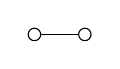
\begin{tikzpicture}[scale=0.8, baseline=-0.5ex]
      \node[graph vertex] (a) at (0,0) {};
      \node[graph vertex] (b) at (0.8,0) {};
      \draw[graph edge] (a) -- (b);
    \end{tikzpicture}
    &
    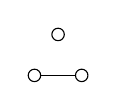
\begin{tikzpicture}[scale=0.8, baseline=-0.5ex]
      \node[graph vertex] (a) at (0,0) {};
      \node[graph vertex] (b) at (0.75,0) {};
      \node[graph vertex] (c) at (0.375,0.65) {};
      \draw[graph edge] (a) -- (b);
    \end{tikzpicture}
    &
    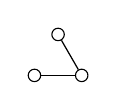
\begin{tikzpicture}[scale=0.8, baseline=-0.5ex]
      \node[graph vertex] (a) at (0,0) {};
      \node[graph vertex] (b) at (0.75,0) {};
      \node[graph vertex] (c) at (0.375,0.65) {};
      \draw[graph edge] (a) -- (b);
      \draw[graph edge] (b) -- (c);
    \end{tikzpicture}
    &
    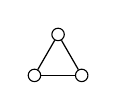
\begin{tikzpicture}[scale=0.8, baseline=-0.5ex]
      \node[graph vertex] (a) at (0,0) {};
      \node[graph vertex] (b) at (0.75,0) {};
      \node[graph vertex] (c) at (0.375,0.65) {};
      \draw[graph edge] (a) -- (b);
      \draw[graph edge] (b) -- (c);
      \draw[graph edge] (c) -- (a);
    \end{tikzpicture}
    \\
    $K_2$ & $T_{\text{one-edge}}$ & $T_{\text{path}}$ & $T_{\triangle}$ \\
    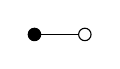
\begin{tikzpicture}[scale=0.8, baseline=-0.5ex]
      \node[graph root] (a) at (0,0) {};
      \node[graph vertex] (b) at (0.8,0) {};
      \draw[graph edge] (a) -- (b);
    \end{tikzpicture}
    &
    
\begin{tikzpicture}[scale=0.8, baseline=-0.5ex]
      \node[graph root] (a) at (0,0) {};
      \node[graph vertex] (b) at (0.8,0) {};
    \end{tikzpicture}
    &
    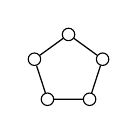
\begin{tikzpicture}[scale=0.7, baseline=-0.5ex]
      \foreach \i/\ang in {1/90,2/18,3/-54,4/-126,5/162} {
        \node[graph vertex] (v\i) at (\ang:0.65) {};
      }
      \draw[graph edge] (v1) -- (v2) -- (v3) -- (v4) -- (v5) -- (v1);
    \end{tikzpicture}
    &
    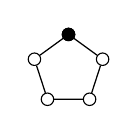
\begin{tikzpicture}[scale=0.7, baseline=-0.5ex]
      \foreach \i/\ang in {1/90,2/18,3/-54,4/-126,5/162} {
        \node[graph vertex] (v\i) at (\ang:0.65) {};
      }
      \node[graph root] at (v1) {};
      \draw[graph edge] (v1) -- (v2) -- (v3) -- (v4) -- (v5) -- (v1);
    \end{tikzpicture}
    \\
    $K_2^\bullet$ & $\overline{K_2}^{\bullet}$ & $C_5$ & $C_5^\bullet$
  \end{tabular}
  \caption{Graphs and rooted flags used in the running examples.  Filled
  vertices are labeled vertices of a flag.}
  \label{fig:small-graphs}
\end{figure}

\subsection{Subflag Densities}

% Once pattern flags have been named, the basic question is simple: if we sample
% a few extra vertices in a larger host flag, what smaller flag do we see?
% The resulting densities are the bridge between finite host flags and
% asymptotic limits.  Along a convergent sequence of larger and larger flags,
% each fixed finite pattern has a limiting density.  Flag algebra manipulates
% those limiting densities symbolically, but every coefficient comes from the
% finite probability definitions below.  This is why the method is well suited
% to machine checking: the coefficients in a certificate are not analytic
% guesses, but rational numbers obtained by finite enumeration.

\paragraph{Single-flag density.}
Let $\sigma$ be a type of size $k$.  For a $\sigma$-flag $A$ of size $m$
(the \emph{pattern flag}) and a $\sigma$-flag $G$ of size $n \geq m$
(the \emph{host flag}), the \emph{induced subflag density} $\den{A}{G}$ is
the probability that a uniformly random $(m-k)$-element subset of
$V(G) \setminus \operatorname{Im}(\theta_G)$, together with the labeled
vertices of $G$, induces a $\sigma$-flag isomorphic to $A$.  Explicitly:
\[
  \den{A}{G}
  \;=\;
  \frac{1}{\binom{n-k}{m-k}}
    \cdot {\Bigl|\Big\{S \subseteq V(G)\setminus \operatorname{Im}(\theta_G)
                  ~\Big|~ |S|=m-k,\;
                  G[S \cup \operatorname{Im}(\theta_G)]
                  \text{ is isomorphic to } A
                  \text{ as a }\sigma\text{-flag}\Big\}\Bigr|}.
\]
This value lies in $[0,1]$ and is invariant under
isomorphism of both $A$ and $G$.

\begin{example}[A rooted pentagon density]
  Let $\sigma$ be the one-vertex type, and let $K_2^\bullet$ be the
  $\sigma$-flag on two vertices in which the unlabeled vertex is adjacent to
  the labeled one.  Let $\overline{K_2}^{\bullet}$ be the corresponding
  non-edge flag.  These flags are shown in \Cref{fig:small-graphs}.  Now root
  a copy of $C_5$ at one of its vertices.  Among the
  four non-root vertices, exactly two are neighbors of the root.  Hence
  \[
    \den{K_2^\bullet}{C_5^\bullet} = \frac{2}{4} = \frac12,
    \qquad
    \den{\overline{K_2}^{\bullet}}{C_5^\bullet} = \frac{2}{4} = \frac12.
  \]
  This tiny example captures the reason flags are useful: a flag remembers
  the local view from a labeled configuration.  The same unrooted pentagon can
  be queried from the perspective of a distinguished vertex, and the algebra
  keeps those conditional densities as named algebraic coordinates rather than
  side comments in prose.
\end{example}

\paragraph{Joint density.}
For pattern $\sigma$-flags $A_1$ of size $m_1$ and $A_2$ of size $m_2$ and a host
$\sigma$-flag $G$ of size $n \geq m_1 + m_2 - k$, the \emph{joint density}
$\den{A_1,A_2}{G}$ is the probability, over a uniformly chosen ordered pair
of disjoint subsets
\[
  S_i \subseteq V(G)\setminus \operatorname{Im}(\theta_G),
  \qquad |S_i|=m_i-k,
\]
that $S_i$ together with the labeled vertices of $G$ induces a
$\sigma$-flag isomorphic to $A_i$, for $i=1,2$.
Joint densities are what make multiplication possible: the product of two
pattern flags is interpreted as the probability that two disjoint samples occur
simultaneously in the same host.  This turns combinatorial double counting
into algebra.

\subsection{The Flag Algebra}

The next step is to stop distinguishing between expressions that have the same
asymptotic meaning.  A small pattern flag $A$ can be counted directly in a
large host flag $G$.  Equally, one can first sample a larger intermediate flag
$B$ inside $G$, then count $A$ inside $B$, and finally average over the choice
of $B$.
These two sampling procedures give the same limiting density.  The flag
algebra builds this sampling-averaging identity into the syntax by quotienting
it out.  As a result, a proof can replace a pattern flag by any sufficiently
large expansion of it, which is exactly the bookkeeping needed by flag algebra
certificates.  This is the same kind of move one makes when quotienting
programs by an equational theory: the quotient removes representation choices
that should not affect observable behavior.

Fix a type $\sigma$ of size $k$.  Let
$\mathbb{R}[\mathcal{F}^\sigma]$ be the free $\mathbb{R}$-module with basis
$\mathcal{F}^\sigma$, i.e., the vector space of finite formal real linear
combinations of $\sigma$-flags.  We also write $A$ for the basis vector
corresponding to a flag $A$.
Define the \emph{zero space} $\mathcal{Z}^\sigma$ as the subspace generated
by all elements of the form
\[
  A - \sum_{B \in \mathcal{F}^\sigma_n} \den{A}{B} \cdot B,
  \qquad \text{for}\ A \in \mathcal{F}^\sigma_m \ \text{and}\ n \geq m.
\]
The \emph{flag algebra} is the quotient module
\[
  \mathcal{A}^\sigma \;=\; \mathbb{R}[\mathcal{F}^\sigma] \,/\, \mathcal{Z}^\sigma.
\]
The zero-space relations express the combinatorial identity that, in a
sufficiently large host flag $G$,
\[
  \den{A}{G}
  =
  \sum_{B \in \mathcal{F}^\sigma_n} \den{A}{B}\,\den{B}{G}.
\]
That is, counting $A$ directly agrees with counting through an intermediate
sample of size $n$.

\paragraph{Multiplication.}
For flags $A_1 \in \mathcal{F}^\sigma_{m_1}$ and
$A_2 \in \mathcal{F}^\sigma_{m_2}$, choose an auxiliary size
$\ell \geq m_1 + m_2 - k$ and set
\[
  [A_1] \cdot [A_2]
  \;=\;
  \sum_{D \in \mathcal{F}^\sigma_\ell} \den{A_1,A_2}{D} \cdot [D]
  \qquad\text{in } \mathcal{A}^\sigma.
\]
The zero-space quotient is what makes this formula independent of the
auxiliary size $\ell$; it also respects isomorphism classes of the input flags.
Extending bilinearly gives a commutative, associative $\mathbb{R}$-algebra.
The unit is the type flag consisting only of the labeled vertices; we write it
as $\mathbf{1}_\sigma$, and simply as $\mathbf{1}$ when $\sigma=\emptyset$.

\begin{example}[The edge expansion behind Mantel's theorem]
  The simplest useful zero-space relation expands the unlabeled edge $K_2$ (which
  is thus a $\emptyset$-type flag) at
  size $3$.  There are four unlabeled graphs on three vertices: the empty
  graph, the one-edge graph, the two-edge path, and the triangle
  (the latter three are shown in \Cref{fig:small-graphs}).  If an
  edge is sampled uniformly from the three possible vertex pairs, its density
  in these graphs is respectively
  \[
    0,\qquad \frac13,\qquad \frac23,\qquad 1.
  \]
  Thus the quotient identifies
  \[
    K_2
    \;=\;
    \frac13\,T_{\text{one-edge}}
    + \frac23\,T_{\text{path}}
    + T_{\triangle}
    \qquad\text{in } \mathcal{A}^{\emptyset}.
  \]
  Mantel's theorem is the statement that the asymptotic edge density $K_2$ is
  at most $1/2$ in every $K_3$-free graph.  In the flag algebra proof,
  we start with the above equation and then eliminate the triangle term
  using the $K_3$-free hypothesis.  This style of expansion is common in
  flag algebra proofs.  It is also exactly the kind of elementary
  combinatorial bookkeeping that becomes unwieldy in the Lean formalization of
  more complex arguments, including the pentagon proof.  There the coefficients
  are still rational numbers from finite sampling, but there are hundreds of
  them, and every one must be justified inside Lean.
\end{example}

\subsection{Positive Homomorphisms, Semantic Order, and Unlabeling}

The quotient algebra is syntax for density expressions.  To use such an
expression in an extremal argument, we need to say how it is evaluated in a
limiting graph sequence.  That role is played by positive homomorphisms.

\paragraph{Positive homomorphisms.}
Fix a type $\sigma$.  A \emph{positive homomorphism} on
$\mathcal{A}^\sigma$ is an $\mathbb{R}$-algebra homomorphism
$\phi:\mathcal{A}^\sigma \to \mathbb{R}$ such that
$\phi([A]) \geq 0$ for every $\sigma$-flag $A$.  Thus $\phi$ assigns a real
number to each algebra expression, respects addition and multiplication, and
never assigns a negative value to a concrete flag.

In the unlabeled case $\sigma=\emptyset$, positive homomorphisms are exactly
the semantic objects represented by convergent graph sequences.  That is, if
$(G_n)_{n \in \mathbb{N}}$ is a sequence of finite graphs with
$|V(G_n)|\to\infty$ and every density $\den{A}{G_n}$ has a limit, then
\[
  [A]\longmapsto \lim_{n\to\infty}\den{A}{G_n}
\]
extends to a positive homomorphism on $\mathcal{A}^\emptyset$; conversely,
every positive homomorphism on $\mathcal{A}^\emptyset$ arises this way in
Razborov's semantics~\cite{razborov2007flag}.

\paragraph{Semantic non-negativity and order.}
For a fixed type $\sigma$, define the \emph{semantic non-negativity cone}
\[
  \mathcal{C}^\sigma
  =
  \{f \in \mathcal{A}^\sigma
    \mid \phi(f) \geq 0
    \text{ for every positive homomorphism }
    \phi:\mathcal{A}^\sigma\to\mathbb{R}\}.
\]
An element of $\mathcal{C}^\sigma$ is non-negative under every positive
homomorphism of the $\sigma$-flag algebra.  We write
\[
  f \leq_\sigma g
  \qquad\text{when}\qquad
  g-f \in \mathcal{C}^\sigma.
\]
Equivalently, $f\leq_\sigma g$ means that
$\phi(f)\leq\phi(g)$ for every positive homomorphism
$\phi:\mathcal{A}^\sigma\to\mathbb{R}$.  When $\sigma=\emptyset$, we write
$\mathcal{C}$ for $\mathcal{C}^\emptyset$ and omit the subscript from
$\leq_\emptyset$.

\paragraph{Squares and PSD quadratic forms.}
A real symmetric matrix $Q \in \mathbb{R}^{r\times r}$ is \emph{positive
semidefinite} (PSD) if $v^\top Q v\geq 0$ for every real vector
$v \in \mathbb{R}^r$.  The simplest source of elements of
$\mathcal{C}^\sigma$ is a square: if $e\in\mathcal{A}^\sigma$ and $\phi$ is a
positive homomorphism, then
\[
  \phi(e^2)=\phi(e)^2\geq 0.
\]
So $e^2$ is semantically non-negative.  A finite sum
$\sum_i a_i e_i^2$ with $a_i\geq 0$ is non-negative for the same reason.  More
generally, if $Q$ is PSD and $e_1,\ldots,e_r\in\mathcal{A}^\sigma$, then every
positive homomorphism sends
\[
  \sum_{i,j=1}^r Q_{ij}\,e_i e_j
\]
to the real quadratic form $v^\top Q v$ for
$v=(\phi(e_1),\ldots,\phi(e_r))$, which is always non-negative.  So the
above quadratic expression is in $\mathcal{C}^\sigma$.
This is the sense in which flag algebra
proofs use ``sums of squares'': the proof data is a finite quadratic expression
whose value is forced to be a non-negative real number by a PSD matrix.

\paragraph{Downward (unlabeling) operator.}
Labeled algebras (i.e., $\mathcal{A}^\sigma$ with
$\sigma \neq \emptyset$) often give stronger quadratic expressions because
labels record local structure.  The final extremal statement, however, is
usually about unlabeled graphs (i.e., flags for the empty type), such as an
upper bound on the density of $C_5$ in triangle-free graphs.  The downward
operator is the averaging map that forgets the labels with the correct
normalization, converting a labeled algebra expression into an unlabeled one.

For a $\sigma$-flag $A=(G,\theta_A)$ of size $m$ (type of size $k$), let
$A|_\emptyset$ be the underlying graph $G$, which is also a flag for the empty
type.  Following Razborov's definition~\cite{razborov2007flag}, the
\emph{downward operator} does not sum over all labelings of $G$.  Instead, it
forgets the labels and multiplies by the probability that a random injection
of the type vertices would recover the same labeled flag.  More precisely,
define
\[
  q_\sigma(A)
  \;=\;
  \frac{
    \bigl|\{\theta' : [k]\hookrightarrow V(G)
       \mid \theta' \text{ embeds }\sigma\text{ into }G
       \text{ and } (G,\theta')\cong_\sigma A\}\bigr|}
       {m(m-1)\cdots(m-k+1)}.
\]
Then
\[
  \llbracket A \rrbracket_\sigma
  \;=\;
  q_\sigma(A)\cdot A|_\emptyset,
\]
extended linearly to all of $\mathcal{A}^\sigma$.

\begin{theorem}[Razborov~{\cite{razborov2007flag}}]
  \label{thm:sdp-nonneg}
  For any type $\sigma$, elements $e_1,\ldots,e_r \in \mathcal{A}^\sigma$,
  and positive semidefinite matrix $Q \in \mathbb{R}^{r\times r}$,
  \[
    \Bigl\llbracket \sum_{i,j=1}^r Q_{ij}\, e_i\, e_j \Bigr\rrbracket_\sigma
    \;\in\; \mathcal{C}.
  \]
\end{theorem}

The conclusion says that every positive homomorphism on
$\mathcal{A}^\emptyset$ evaluates the downward-averaged quadratic expression
as a non-negative real number.  This is the engine behind flag algebra bounds
based on positive semidefinite matrices.  Given a target element
$x_0 \in \mathcal{A}^\emptyset$ and a claimed bound $c \in \mathbb{R}$, if
one exhibits a PSD matrix $Q$ and elements $e_i \in \mathcal{A}^\sigma$ such
that
\[
  c \cdot \mathbf{1} - x_0
  \;=\;
  \Bigl\llbracket \sum_{i,j} Q_{ij}\, e_i\, e_j \Bigr\rrbracket_\sigma,
\]
then $c\cdot\mathbf{1}-x_0\in\mathcal{C}$, so
$\phi(x_0) \leq c$ for every positive homomorphism
$\phi:\mathcal{A}^\emptyset\to\mathbb{R}$.

\subsection{Turán Densities and the Pentagon Problem}

We can now connect the algebra back to the combinatorial problems that motivate
it.  Here $H$ is an unlabeled forbidden graph and $P$ is an unlabeled target
graph.  The finite graphs being optimized over are $H$-free, meaning that they
contain no induced subgraph isomorphic to $H$, and the target statistic is the
induced density of $P$.

In the algebraic certificate used in this paper, the forbidden-graph
assumption is represented as a condition on positive homomorphisms.  Being
$H$-free is equivalent to having zero induced density of $H$, so we restrict
attention to positive homomorphisms $\phi:\mathcal{A}^\emptyset\to\mathbb{R}$
satisfying
\[
  \phi([H])=0.
\]
Every convergent sequence of $H$-free graphs gives such a homomorphism.  For
$H=K_3$, the condition says precisely that the limiting triangle density is
zero.

To distinguish this from the type-indexed order $\leq_\sigma$, for
$f,g\in\mathcal{A}^\emptyset$ write
\[
  f \forbLE{H} g
\]
when $\phi(f)\leq\phi(g)$ for every positive homomorphism
$\phi:\mathcal{A}^\emptyset\to\mathbb{R}$ satisfying
$\phi([H])=0$.  Equivalently, $g-f$ evaluates to a non-negative real number in
every positive homomorphism satisfying the forbidden-graph condition
$\phi([H])=0$.
Thus an upper-bound proof for the target graph $P$ aims to establish
\[
  [P] \forbLE{H} c\cdot\mathbf{1}.
\]
The finite proof data usually combines three ingredients already defined
above: zero-space relations expand expressions to a common size, PSD quadratic
forms provide semantically non-negative terms, and the downward operator turns
labeled quadratic terms into unlabeled ones.

\paragraph{Generalized Turán density.}
For an unlabeled target graph $P$ and an unlabeled forbidden graph $H$, the
\emph{generalized Turán density} is
\[
  \tdensity{P}{H}
  \;=\;
  \lim_{n\to\infty}
  \frac{1}{\binom{n}{|V(P)|}} \cdot
    {\max\Bigl\{|\text{induced copies of }P\text{ in }G|
                   ~\Big|~ |V(G)|=n \text{ and } G \text{ is }H\text{-free}\Bigr\}}.
\]
For the complete forbidden graph used in the certificate, the semantic
inequality $[P] \forbLE{H} c\cdot\mathbf{1}$ implies
$\tdensity{P}{H}\leq c$.  A matching construction gives the reverse
inequality when the claimed value is sharp.

\paragraph{The Erd\H{o}s pentagon problem.}
The problem asks for $\tdensity{C_5}{K_3}$: the maximum density of
pentagons in triangle-free graphs.  The answer $24/625$ was proved
independently by Grzesik~\cite{grzesik2012} and by Hatami, Hladk\'y, Kr\'al,
Norine, and Razborov~\cite{hatami2012}.  It is achieved by the blow-up of
$C_5$ (partition $n$ vertices into five nearly-equal groups and add all edges
between consecutive groups in the cycle).  We use this theorem as the main
case study throughout the paper, as it involves the full proof-engineering
stack: abstract structure, extensional finite counting, data-heavy density
computation (thousands of rational values over 5-vertex graphs), and heavy
algebraic bookkeeping.


\section{The Mathematical Specification}
\label{sec:abstract}

The specification layer of our Lean formalization gives flag algebras a
typed mathematical interface that is reusable across different extremal
problems.  This section describes the choices we made for that interface.
We are reporting choices, not contributions: each choice has a coherent
alternative, and on at least one of them we do not know which is preferable.

\paragraph{A design choice, not an enabling condition.}
In our predicate-based design, the forbidden-subgraph assumption is deferred
to a parameter on the semantic order rather than baked into a universal theory
at the outset.  In Razborov's original presentation~\cite{razborov2007flag},
the forbidden subgraph is specified by a universal first-order theory chosen
when the algebra is set up; both designs can express the same mathematical
statements.  A consequence---not an enabling condition---of our choice is
that random-extension theorems become the definitional content of the
forbidden-subgraph relation, rather than serving only as an analytic
ingredient inside a fixed theory.  What differs between the two designs is
which intermediate lemmas are reusable across choices of constraint, and how
many compatibility theorems must be reproved when a new forbidden graph is
introduced.  Whether predicate-deferral is preferable to Razborov's
universal-theory specification is a tradeoff we report on, not one we resolve.

\paragraph{What this section reports.}
In informal arguments, the same symbol freely denotes a concrete graph, its
isomorphism class, a formal linear combination of flags, an element of the
quotient algebra, or a real value assigned by a positive homomorphism; the
transitions between these roles are implicit.  In Lean they are explicit:
each role is a distinct type, and each transition is a map that must be
proved compatible with the relevant equivalence relations and algebraic
operations.  The specification layer provides those maps and their
compatibility theorems, so that every subsequent certificate proof can work
at the algebra level without re-establishing the soundness of the surrounding
framework.

The structure of the specification follows Razborov's mathematical
presentation.  Flags are quotients of labeled graphs by isomorphism.  Their
densities are formalized as a sampling semantics: the probability that a
uniformly random induced subgraph of a host graph is isomorphic to a given
flag.  The flag algebra is a further quotient, of the free real vector space
on flags, by expansion laws that identify a small flag with its expected
density expansion to a collection of larger flags.  Positive homomorphisms
are the models of that equational theory.  Razborov's random-extension
theorem, formalized using Mathlib's Prokhorov compactness theorem, connects
the standard empty-typed level with the typed levels: every positive
homomorphism $\phi$ on the empty-typed algebra extends to a probability
measure $\mathbb{P}^{\phi}$ on the space of $\sigma$-typed positive
homomorphisms for any $\sigma$.  This measure-theoretic result is the
foundation on which the forbidden-subgraph predicate $\forbLES{\sigma}{H}$
rests.  The transfer theorem
\lean{generalizedTuranDensity\_le\_of\_forbidLE} then reduces a Tur\'an
density bound to a single empty-typed semantic inequality $[P] \forbLE{H}
c\cdot\mathbf{1}$ in the ambient algebra.  Any proof of that inequality,
however it is assembled, immediately yields the bound $\tdensity{P}{H}\leq
c$; and all the abstract-layer results about products, quadratic forms, and
the downward operator carry over to every forbidden graph without reproof.
Code snippets are lightly rendered in ASCII when the Lean source uses Unicode
notation; the names and fields match the implementation.

\subsection{Types and Flags in Lean}

The central representation problem is this: the mathematics works with
isomorphism classes of labeled graphs, but a type theory only knows about
concrete terms.  A function on flags must not depend on which representative
was chosen from an isomorphism class, yet the proof assistant cannot verify
this without being told explicitly.  The implementation resolves this tension
in three steps: build a concrete representation, quotient by the relevant
equivalence, and carry enough size information for later algebraic operations.

The finite set $[k]$ is represented by \lean{Fin k}, and Mathlib's
\lean{SimpleGraph V} is the type of simple undirected graphs with vertex type
\lean{V}.  A flag type $\sigma$ of size $k$ is therefore a
\lean{SimpleGraph (Fin k)}; the abbreviation
\begin{lstlisting}
abbrev FlagType := SimpleGraph
\end{lstlisting}
gives it a more suggestive name without introducing a new structure.  In Lean,
\lean{abbrev} declares a definition that the type-checker treats as a
transparent alias, roughly analogous to a reducible \lean{Definition} in Rocq.
Before quotienting, a concrete $\sigma$-flag is:
\begin{lstlisting}
structure LabeledGraph (sigma : FlagType T) (V : Type) where
  graph      : SimpleGraph V
  type_embed : sigma ->g graph
\end{lstlisting}
The field \lean{type\_embed} is a Mathlib graph embedding (written \lean{->g}
in the source): an injective vertex map that both preserves and reflects
adjacency.  Its image is an induced copy of $\sigma$, exactly the labeling map
$\theta_A$ in a flag $A = (G, \theta_A)$.

Two \lean{LabeledGraph} values represent the same flag when there is a graph
isomorphism between their ambient graphs that commutes with both embeddings of
$\sigma$.  This is the setoid \lean{labeledGraphSetoid}, and the flag type is
its quotient:
\begin{lstlisting}
def Flag (sigma : FlagType T) (V : Type) : Type :=
  Quotient (labeledGraphSetoid sigma V)
\end{lstlisting}
This design follows Razborov's original presentation, in which flags are
isomorphism classes from the outset.  The alternative---choosing a canonical
representative for each isomorphism class---is common in computational
implementations and avoids quotient eliminators entirely.  We did not take that
route because it would attach representation-specific side conditions to every
algebraic lemma.  The cost of working with quotients is instead a recurring
proof obligation: in Lean, every function \emph{from} a quotient type must be
constructed via \lean{Quotient.lift}, which requires an explicit proof that the
function respects the equivalence relation.  We say more about the cost of
this choice in Section~\ref{sec:obstacles}.

Expansion identities and products range over auxiliary sizes, and the final
algebraic element must be shown independent of those auxiliary choices.  Two
thin wrappers make the ambient vertex count explicit:
\begin{lstlisting}
abbrev FlagWithSize (sigma : FlagType (Fin n0)) (n : N) :=
  Flag sigma (Fin n)

def FinFlag (sigma : FlagType (Fin n0)) : Type :=
  Sigma (fun n : N => FlagWithSize sigma n)
\end{lstlisting}
Here \lean{Sigma} is Lean's dependent pair type (written \lean{sigT} in Rocq).
\lean{FlagWithSize sigma n} implements $\mathcal{F}^\sigma_n$, and
\lean{FinFlag sigma} is the all-size disjoint union that serves as the basis
of the free vector space.  The first component of a \lean{FinFlag} records the
ambient size; later quotient theorems prove that the algebraic element it
represents is independent of whichever auxiliary size was chosen in
intermediate computations.

\subsection{Densities as Sampling Semantics}

The next viewpoint is probabilistic.  A density $\den{F}{G}$ is the value of a
finite sampling experiment: keep the type vertices fixed, sample the remaining
vertices of the host graph, and observe the induced flag.  This reading is
important for certification.  The SDP search manipulates algebraic density
expressions, while Lean grounds each expression in a finite sample space and a
finite count.

The implementation in \lean{FlagAlgebra/SubflagListDensity.lean} defines this
sampling semantics uniformly for lists of requested flags.  This avoids a
separate theory for one-flag densities, pair densities, and triple densities.
At the representative level, \lean{LabeledSubgraphList} records the sampled
subgraphs of a host.  The main well-formedness conditions are:
\begin{lstlisting}
LabeledSubgraphList.IsInduced
predDisjointLabeledSubgraphList
predIsoLabeledHl
\end{lstlisting}
They say that each sample is induced, that independently sampled flags overlap
only in the shared type vertices, and that the observed subgraphs have the
requested flag-isomorphism type.  The density is the rational value of that
experiment:
\begin{lstlisting}
def labeledSubgraphListDensity (Hl : LabeledGraphList sigma t Vl)
    (G : LabeledGraph sigma W) : Q :=
  labeledSubgraphListCount Hl G /
    multinomialCoefficient r_list (G.size - sigma.size)
\end{lstlisting}
The denominator is the size of the finite sample space for the additional,
unlabeled vertices.  The quotient lift is justified by
\lean{labeledSubgraphListDensity\_respect\_eqv}: replacing the requested flags
or the host by isomorphic labeled graphs gives the same rational number.  This
is the first recurring pattern of the section: the quotient remains the
specification, and computations over representatives are admitted only after an
invariance proof.

The single- and two-flag densities used by the algebra are arity-specialized
views of this same semantics:
\begin{lstlisting}
def flagDensity1 (F : Flag sigma U) (G : Flag sigma W) : Q :=
  flagListDensity [F] G

def flagDensity2 (F1 : Flag sigma U1) (F2 : Flag sigma U2)
    (G : Flag sigma W) : Q :=
  flagListDensity [F1, F2] G
\end{lstlisting}
The Lean source names these constants with Unicode subscripted numerals; the
displayed code uses ASCII names only for portability.  Conceptually,
\lean{flagDensity1} is the induced
subflag density $\den{F}{G}$, while \lean{flagDensity2} is the joint density
that makes multiplication possible.

\subsection{The Algebra as an Equational Theory}

The flag algebra itself is the point where finite sampling expressions become
an equational calculus.  Paper proofs freely replace a small flag by its
expected expansion in a larger host size.  In Lean this replacement is not a
simplification rule; it is the defining relation of the quotient algebra.  We
start with the free real vector space on all finite $\sigma$-flags:
\begin{lstlisting}
abbrev FlagVector (sigma : FlagType (Fin n0)) : Type :=
  FinFlag sigma ->0 R

def unitVector (F : FinFlag sigma) : FlagVector sigma :=
  Finsupp.single F 1
\end{lstlisting}
Here \lean{->0} is Mathlib's type of finitely supported functions.  The
expansion law identifies a basis flag with its density expansion at any larger
size:
\begin{lstlisting}
def densityFlagSum (F : FinFlag sigma) (ell : N) : FlagVector sigma :=
  sum F' : FlagWithSize sigma ell,
    flagDensity1 F.2 F' * unitVector <ell, F'>

def zeroElement (F : FinFlag sigma) (ell : N) : FlagVector sigma :=
  unitVector F - densityFlagSum F ell

def ZeroSpace (sigma : FlagType (Fin n0)) : Submodule R (FlagVector sigma) :=
  Submodule.span R (zeroSet sigma)
\end{lstlisting}
The \lean{zeroSet} records only size choices satisfying \lean{F.1 <= ell}; the
snippet suppresses that guard to foreground the algebraic shape.  The quotient
then says that two formal linear combinations are equal when their difference
is generated by expansion laws:
\begin{lstlisting}
def flagVectorEqv (f g : FlagVector sigma) : Prop :=
  f - g in ZeroSpace sigma

abbrev FlagAlgebra (sigma : FlagType (Fin n0)) : Type :=
  Quotient (flagVectorSetoid sigma)
\end{lstlisting}
This quotient is the semantic bridge from formal linear combinations to
density expressions: a small flag and its larger-size expansion become the
same algebra element.

Multiplication is defined by joint sampling.  On basis elements, the product is
first computed at an auxiliary output size:
\begin{lstlisting}
def flagMulWithSize (F F' : FinFlag sigma) (ell : N) : FlagVector sigma :=
  sum G : FlagWithSize sigma ell,
    flagDensity2 F.2 F'.2 G * unitVector <ell, G>
\end{lstlisting}
The theorem \lean{flagMulWithSize\_indep\_on\_size} proves that any two large
enough choices of \lean{ell} are equivalent modulo the zero space.  Only after
that proof do we lift multiplication to \lean{FlagAlgebra sigma} and build its
commutative ring structure.  The commutativity, associativity, unit laws, and
quotient-compatibility proofs are therefore part of the mathematical content:
they show that the finite sampling semantics supports the symbolic calculus
used by certificates.

\subsection{Positive Homomorphisms as Models}

The next shift is from finite experiments to asymptotic semantics.  Positive
homomorphisms are the models of the equational theory: they assign a real value
to every algebra expression, preserve the algebra operations, and send every
concrete flag to a non-negative number.  In
\lean{FlagAlgebra/PositiveHom.lean} they are implemented as a subtype of real
algebra homomorphisms:
\begin{lstlisting}
abbrev Hom (sigma : FlagType (Fin n0)) :=
  FlagAlgebra sigma ->a[R] R

def PositiveHom (sigma : FlagType (Fin n0)) : Type :=
  { phi : Hom sigma // forall F : FinFlag sigma,
      phi [[unitVector F]] >= 0 }
\end{lstlisting}
The semantic cone is the set of expressions non-negative in all such models:
\begin{lstlisting}
def semanticCone (sigma : FlagType (Fin n0)) : Set (FlagAlgebra sigma) :=
  { f | forall phi : PositiveHom sigma, phi f >= 0 }
\end{lstlisting}
Thus the order on \lean{FlagAlgebra sigma} is a semantic validity relation, not
a syntactic ordering on coefficients.  An inequality $f\leq g$ means that
every positive homomorphism evaluates $f$ no larger than $g$.

The downward operator, implemented in \lean{FlagAlgebra/FlagOperators.lean},
is the bridge from typed algebras back to the empty-typed algebra:
\begin{lstlisting}
def downward : FlagAlgebra sigma -> FlagAlgebra emptyType := ...

notation "[[" f "]]0" => downward f
\end{lstlisting}
It is not just a forgetful map.  The definition includes Razborov's
normalizing factor, and the lift to the quotient proves that averaging over
label placements respects the expansion equations.  This is one of the places
where the formalization exposes an invariant that paper notation usually hides
inside the brackets $\llbracket-\rrbracket_\sigma$.

SDP certificates enter through a compact semantic theorem about quadratic
forms:
\begin{lstlisting}
def flagQuadraticForm (M : Matrix (Fin n) (Fin n) R)
    (v : Fin n -> FlagAlgebra sigma) : FlagAlgebra sigma :=
  sum i, sum j, M i j * (v i * v j)

theorem flagQuadraticForm_nonneg
    (M : Matrix (Fin n) (Fin n) R) (hM : M.PosSemidef)
    (v : Fin n -> FlagAlgebra sigma) :
    flagQuadraticForm M v >= 0

theorem flagQuadraticForm_downward_nonneg
    (hM : M.PosSemidef) (v : Fin n -> FlagAlgebra sigma) :
    [[flagQuadraticForm M v]]0 >= 0
\end{lstlisting}
This is the abstraction barrier for external SDP search.  The search procedure
may propose a matrix, but the checked artifact is a theorem in the semantic
preorder: if Lean verifies the matrix is positive semidefinite, then every
typed positive homomorphism evaluates the corresponding quadratic form
non-negatively, and every empty-typed positive homomorphism evaluates its
downward average non-negatively.

\subsection{Forbidden Graphs as Assumptions, Not New Theories}
\label{sec:forbidden}

The last specification choice is about modularity.  In pen-and-paper flag
algebra proofs, one often works as if there were a separate theory of
$H$-free graphs, with the density of $H$ set to zero from the start.  That is
convenient on paper but a poor formal interface: every forbidden graph would
generate a new quotient theory and a new family of compatibility lemmas.  We
instead keep one ambient flag algebra and put the forbidden condition into
the semantic order.

The predicate is \lean{forbidLE}, in \lean{Forbid/Basic.lean}:
\begin{lstlisting}
def forbidLE (H : FinFlag emptyType) (f g : FlagAlgebra sigma) : Prop :=
  forall (phi0 : PositiveHom emptyType), phi0 <sigma>0 > 0 ->
    phi0 [[unitVector H]] = 0 ->
    P[phi0] {phi | phi f <= phi g} = 1
\end{lstlisting}
For $f,g\in\mathcal{A}^\sigma$, the mathematical relation
$f \forbLES{\sigma}{H} g$ is represented in Lean by this predicate.  It says:
for every empty-typed positive homomorphism $\phi_0$ in which $H$ has density
zero, almost every random $\sigma$-typed extension $\phi$ satisfies
$\phi(f)\leq\phi(g)$.  The side condition \lean{phi0 <sigma>0 > 0} records
that the type $\sigma$ can actually be sampled.  When $\sigma=\emptyset$, this
reduces to the untyped relation, which we write as $f \forbLE{H} g$ in the
paper.

The probability measure $\mathbb{P}^{\phi_0}$ used in this definition is
the most analytic part of the specification layer.  In
\lean{FlagAlgebra/RandomHom.lean}, the code follows Razborov's random-extension
theorem: approximate $\phi_0$ by growing untyped flag sequences, pass to a
subsequential limit of probability measures on the typed density space using
Mathlib's Prokhorov infrastructure, prove that the limit is supported on
positive homomorphisms, and then view it as a probability measure on
\lean{PositiveHomSpace sigma}.  The resulting theorem is:
\begin{lstlisting}
theorem exists_probMeasure_extend_emptyType_positiveHom
    (h_sigma : phi0 <sigma>0 > 0) :
  exists P : ProbabilityMeasure (PositiveHomSpace sigma),
    forall f : FlagAlgebra sigma,
      integral (fun phi => phi f) P =
        phi0 [[f]]0 / phi0 [[(1 : FlagAlgebra sigma)]]0
\end{lstlisting}
This theorem explains why the formalization needs measure theory.  The
downward operator gives the expectation of typed random extensions, so a
forbidden-subgraph assumption stated at the empty-typed level must be
transported through almost-sure statements about typed extensions.  This is
the consequence we mentioned at the start of the section: in the
predicate-based design, random extensions are the definitional content of the
forbidden-subgraph relation, not merely an analytic ingredient supporting a
fixed universal theory.

The final transfer theorem, in \lean{Forbid/TuranDensity.lean}, has the shape
needed by certificate proofs:
\begin{lstlisting}
theorem generalizedTuranDensity_le_of_forbidLE
    (hc : 0 <= c) (h : F.toFlagAlgebra <=[H.toFinFlag] c (*@$\bullet$@*) 1) :
    generalizedTuranDensity H F <= c
\end{lstlisting}
The Lean constant takes the forbidden graph first and the target graph
second: \lean{generalizedTuranDensity H F} is the maximum density of $F$ in
$H$-free graphs, written mathematically in this paper as $\tdensity{F}{H}$.
Here the inequality is empty-typed, so the paper notation is
$F.\lean{toFlagAlgebra} \forbLE{H} c\mathbf{1}$.
The Lean notation \lean{<=[H.toFinFlag]} is the concrete syntax for the same
\lean{forbidLE} predicate.  Once this semantic inequality is checked, the
asymptotic extremal bound follows.  This is the main payoff of the
specification layer: a concrete certificate proof can be assembled from finite
counting, PSD non-negativity, and algebraic rewriting, while the passage from
that certificate to a Tur\'an-density theorem is handled once and reused.


\section{Engineering Obstacles}
\label{sec:obstacles}

The specification layer of Section~\ref{sec:abstract} exposed several
engineering obstacles that we report here as obstacles rather than design
principles.  Three of them follow from Lean~4's intensional type theory and
its typeclass mechanism: quotient eliminators carry recurring compatibility
proofs; size-changing combinatorial operations produce dependent-type
transports; and \lean{Fintype} instances synthesized through different
elaboration paths are extensionally but not definitionally equal.  A fourth
obstacle, function extensionality, is mathematically benign but appears at
every step that relates a function-level equality to a pointwise one.  We
describe the obstacles, the mitigations we used, and where the open ends
remain.  The point is not the particular workarounds; it is that an
intensional type theory makes these obstacles visible at the boundaries of
quotient, dependent-type, and finite-enumeration constructions, and someone
formalizing similar material should expect to face them.

\subsection{Quotient Eliminators and Their Recurring Cost}

Both \lean{Flag} and \lean{FlagAlgebra} are quotients, so any function
\emph{from} them or equality \emph{in} them must go through
\lean{Quotient.lift} or \lean{Quotient.sound}.  \lean{Quotient.lift} requires
a proof that the function respects the equivalence relation;
\lean{Quotient.sound} requires producing a witness of the relation for each
equality goal.

The adequacy theorems in Section~\ref{sec:bridge} illustrate the cost.
To state that \lean{Sym2Graph.toFlag} is inverse to
\lean{Flag.toSym2EmptyTypedFlag}, one cannot simply compute both sides to the
same normal form; the map out of the quotient must go through an eliminator:
\begin{lstlisting}
def Sym2EmptyTypedFlag.toFlag (F : Sym2EmptyTypedFlag n) : Flag emptyType (Fin n) :=
  Quotient.lift Sym2Graph.toFlag Sym2Graph.toFlag_respect_eqv F
\end{lstlisting}
The \lean{toFlag\_respect\_eqv} proof---showing that isomorphic
\lean{Sym2Graph} values map to the same \lean{Flag}---is not automatic; it
required \lean{Quotient.sound} applied to a graph isomorphism witness
assembled from the concrete data.  This is exactly the kind of compatibility
proof that ordinary mathematical notation suppresses.

The recurring cost of carrying \lean{Quotient} eliminators through the
development is real.  A design built around canonical representatives from the
start would not pay this cost, but it would attach representation-specific
side conditions to every algebraic lemma; we chose the quotient design to keep
the specification close to Razborov's mathematics and accept the eliminator
overhead.  Whether the alternative would have been more economical overall is
a tradeoff we cannot evaluate from this vantage point.

\subsection{Dependent-Type Transports from Size-Changing Operations}

Flag algebra operations change the vertex count of flags: the product of a
size-$m_1$ and a size-$m_2$ flag lives at size $\ell \geq m_1 + m_2 - k$.  In
the formalization, the product of basis elements is computed as a sum over
all size-$\ell$ flags.  To show this is well-defined on the quotient (i.e.,
independent of $\ell$), one proves \lean{flagMulWithSize\_indep\_on\_size}.
Its hypotheses say that both output sizes are large enough, and its proof has
to relate sums over \lean{FlagWithSize sigma ell} and
\lean{FlagWithSize sigma ell'}, which are definitionally distinct types even
when the corresponding mathematical sets are connected by expansion.

The same issue arises internally when collecting the flags for the
multiplication sum.  A \lean{FlagList sigma t Vl} (a $t$-tuple of flags with
type family $Vl$) changes type when a new flag is inserted: the result has
type \lean{FlagList sigma (t+1) (listTypeInsert Vl W)}.  Because
\lean{listTypeInsert Vl W} is not definitionally equal to any pre-existing
type family, relating the old and new lists requires \emph{heterogeneous
equality} (\lean{HEq}):
\begin{lstlisting}
theorem flagList_HEq
    (h_Vl_eq : Vl' = Vl)
    (h_Fl_eq : forall i, Fl i = cast (Flag.type_eq h_Vl_eq i) (Fl' i))
    : HEq Fl Fl'
\end{lstlisting}
The \lean{cast} calls are explicit coercions through propositional equality
proofs; they are the formalization's acknowledgment that two types are equal
only up to a proof, not by computation.

Similarly, even if two indices $i$ and $i'$ into a flag list are
propositionally equal ($i = i'$), the types \lean{Flag sigma (Vl i)} and
\lean{Flag sigma (Vl i')} are not definitionally equal, forcing the use of
heterogeneous equality:
\begin{lstlisting}
theorem flaglist_heq_of_idx_eq {i i' : Fin t} (h : i = i')
    : HEq (Fl i) (Fl i') := by subst h; rfl
\end{lstlisting}
This pervasive use of \lean{HEq} and \lean{cast} propagates through the entire
density computation infrastructure: every operation that crosses a size
boundary must carry explicit propositional equality evidence.  Our
\emph{mitigation} was to isolate each size-change obligation in a small named
lemma---examples are \lean{flagList\_HEq},
\lean{flaglist\_heq\_of\_idx\_eq}, and \lean{flagListDensity\_HEq\_eq}---so
that high-level proofs invoke clean invariance statements while the transport
details remain in the small layer where they belong.

\subsection{Function Extensionality and Proof-Valued Fields}

In Lean~4's intensional type theory, function extensionality
($(\forall x,\, f\,x = g\,x) \Rightarrow f = g$) is not definitional but is
available as an axiom (\lean{funext}, derived from \lean{propext}).  This
creates friction wherever the formalization must relate a function-level
equality (such as a type embedding) to a pointwise equality (the embedding's
behavior on individual vertices).  For example, constructing a labeled-graph
isomorphism from a vertex map $\zeta$ requires reassembling pointwise
information back into a function:
\begin{lstlisting}
have h_emb : forall t : T, zeta (G0'.type_embed t) = G1'.type_embed t := ...
let iso : G0'.coe =~f G1'.coe := { ..., type_preserve := funext h_emb }
\end{lstlisting}
Without \lean{funext} as an axiom, the \lean{type\_preserve} field could not
be filled.

Proof-valued structure fields create a related difficulty.  The
\lean{Sym2Graph} type carries a field
\lean{edges\_valid : forall e in edges, not e.IsDiag}; two \lean{Sym2Graph}
values with the same edge set but different proof terms for
\lean{edges\_valid} are propositionally equal (by proof irrelevance) but not
definitionally equal.  Comparing \lean{Sym2Graph} values in the adequacy
theorems therefore requires \lean{proof\_irrel\_heq} at every such field:
\begin{lstlisting}
theorem Sym2Graph.toLabeledGraph_toSym2Graph_eq (G : Sym2Graph n) :
    G.toLabeledGraph.toSym2Graph = G := by
  congr  -- reduces to field equalities
  ...
  exact proof_irrel_heq _ _  -- edge validity field
\end{lstlisting}

\subsection{Fintype Instance Conflicts}
\label{sec:fintype}

The fourth obstacle is the most pervasive in the counting layer.  Sets defined
by set-builder notation $\{x \mid P\ x\}$ have type \lean{Set T}, which is
\lean{Finite} whenever \lean{T} is a \lean{Fintype}, but does not
automatically carry a \lean{Fintype} instance.  Many Mathlib lemmas about
cardinality (\lean{Fintype.card}, \lean{Finset.card\_univ},
\lean{Fintype.card\_congr}) require \lean{Fintype}, not merely \lean{Finite}.
The elaborator infers \lean{Fintype} instances automatically, but in a
development with multiple overlapping constructions (quotient types, embedded
subgraphs, partial-function spaces), the same type can receive different
\lean{Fintype} instances from different elaboration paths.  When two
instances do not reduce to the same term definitionally, the kernel rejects
the goal even if the instances are provably equal.

The mitigation is to bind the intended \lean{Fintype} instance immediately
after naming a finite set:
\begin{lstlisting}
let hS0 : Fintype S0 := Fintype.ofFinite S0
let hS1 : Fintype S1 := Fintype.ofFinite S1
have card_eq : Fintype.card S0 = Fintype.card S1 :=
  Fintype.card_congr h_iso_S0_S1
\end{lstlisting}
This pattern appears repeatedly in \lean{SubflagListDensity.lean}: for the
quotient-respect lemma for list densities, for permutation of sampled flags,
and for insertion of an empty flag.  Without the explicit \lean{let} bindings,
Lean can synthesize a \lean{Fintype} for each set through a different path at
each use, and \lean{Fintype.card\_congr} no longer sees the two cardinalities
as referring to the same enumeration terms.  A similar explicit
\lean{Fintype.ofFinite} construction is used in \lean{FlagOperators.lean} for
the isomorphism set with a fixed underlying graph.

For parameterized types such as injections \lean{Embedding V W} and
equivalences \lean{Equiv V W}, Lean can synthesize \lean{Fintype} instances in
multiple ways depending on which prior instances are in scope.  In
\lean{Compute/Basic.lean}, where \lean{Fintype} instances for these types are
defined, the elaborator had to be given explicit guidance via
\lean{@Finset.univ}:
\begin{lstlisting}
instance : Fintype (Embedding V W) :=
  { elems := (@Finset.univ (V -> W)).filterMap ..., ... }

instance : Fintype (G1 ->g G2) :=
  { elems := (@Finset.univ (Embedding V W)).filterMap ..., ... }
\end{lstlisting}
The graph-embedding and graph-isomorphism instances are built by filtering
finite enumerations of simpler function or equivalence types.  The explicit
\lean{@Finset.univ} keeps the intended enumeration visible to the elaborator,
instead of relying on typeclass search to rediscover it in a later goal.
A related issue arose for dependent function types indexed by a small finite
type, where Lean's typeclass search does not look through \lean{match}
expressions inside type-valued functions; the \lean{FintypeList} typeclass
threads \lean{Fintype} instances per component explicitly to compensate.

\paragraph{What remains open.}
Not all intensionality obstacles were resolved.  The most significant gap is
in \lean{Forbid/Basic.lean}: several strengthening lemmas about recovering
representative-level information from quotient-level forbidden equalities
remain as commented proof sketches, not as imported declarations or trusted
axioms.  For example, one would like a general theorem saying that if a
basis vector is zero under the forbidden equality relation, then the
corresponding unlabeled flag has positive density of the forbidden graph.
Proving such a statement requires careful reasoning about how zero-space
relations interact with individual representatives.  This is not needed for
the main case studies---\lean{Mantel\_theorem} and \lean{ErdosPentagon\_Turan}
are proved without those sketches---but it marks a natural direction for
making the \lean{forbidLE} framework more convenient for future applications.


\section{The Bridge from Specification to Evaluable Proof}
\label{sec:bridge}

The specification of Section~\ref{sec:abstract} is mathematically right and
operationally wrong: \lean{flagDensity} is defined via non-constructive
quotients, the relevant \lean{Decidable} instances are not available
directly, and the abstract layer has no notion of an external SDP solver.
The bridge layer turns the specification into something a concrete proof can
use.  It has four parts: a reflection layer that connects the abstract
definitions to a computable graph type via adequacy theorems; SDP-certificate
verification via LDL$^\top$ decomposition over $\Q$; a tactic layer that
automates the recurring algebraic bookkeeping; and an API layer that packages
all of the above behind a small interface used by the case studies.  We
report each part as something we had to build rather than as a contribution
in its own right.

\subsection{Proof by Reflection in ITP}

The proof-by-reflection pattern in interactive theorem proving has three
components: (1) a \emph{concrete representation} over which a decision
procedure can evaluate; (2) an \emph{adequacy theorem} proving that the
decision procedure is sound with respect to the abstract definition; and (3)
a \emph{decision procedure} (the evaluator) that, given the concrete
representation, produces a Boolean answer which \lean{decide} converts into a
proof.  Our architecture applies this pattern at multiple granularities.  The
pattern itself is decades old; what we report here is the specific failure
mode it exhibits when the abstract specification is built from quotient types,
and how we worked around it.

\subsection{Concrete Graph Representations}

We introduce \lean{Sym2Graph n} in
\lean{LeanFlagAlgebras.FlagAlgebra.Compute.Basic}:
\begin{lstlisting}
structure Sym2Graph (n : N) where
  edges       : Finset (Sym2 (Fin n))
  edges_valid : forall e in edges, not e.IsDiag
\end{lstlisting}
This represents a graph on $\{0,\ldots,n-1\}$ as a finite set of unordered
non-diagonal pairs.  Unlike \lean{SimpleGraph (Fin n)} (which uses a
\lean{Prop}-valued adjacency relation), every operation on \lean{Sym2Graph n}
is computable: membership in \lean{edges} is decidable by \lean{Finset}
membership.  The same file derives the \lean{Fintype} instances needed to
make graph isomorphism decidable:
\begin{lstlisting}
instance : Fintype (G1 ->g G2) := ...   -- graph embeddings
instance : Fintype (G1 =~g G2) := ...   -- graph isomorphisms
instance : Decidable (Nonempty (G =~f G')) := ...  -- flag isomorphism
\end{lstlisting}
These instances enumerate candidates (all injections from $V(G_1)$ to
$V(G_2)$, or all bijections) and filter those that preserve adjacency and
type embeddings.  This reduces ``are these two labeled graphs isomorphic?'' to
a finite, decidable search.

\subsection{From Naive Reflection to Usable Reflection}

The central engineering lesson of the reflection layer is that
\emph{computable} is not the same as \emph{usable}.  A straightforward
reflective design would keep the abstract definitions as close as possible to
the mathematics, make the relevant finite types into \lean{Fintype}s, and ask
\lean{native\_decide} to evaluate density goals by unfolding
\lean{flagDensity}.  This works as a proof of concept, but it is not a viable
compilation strategy for the pentagon proof.  Each density check would then
repeatedly construct finite sets of abstract subgraphs, compare quotient
classes by searching for flag isomorphisms, synthesize overlapping
\lean{Fintype} instances, and carry proof-valued fields through the
evaluator.  The graphs are small, but the proof terms are not: the evaluator
is reducing a proof-relevant encoding of finite combinatorics, not a simple
graph algorithm.

The optimized layer treats reflection more like verified compilation.  The
abstract quotient definitions remain the specification, while the executable
programs in \lean{Compute/FastIso.lean} and \lean{Compute/FlagDensity.lean}
act as compiled code.  The connection between them is established by adequacy
theorems, so changing the implementation of the Boolean checker does not
change the mathematical theorem being proved.

\paragraph{Optimization 1: Boolean isomorphism with early pruning.}
The first bottleneck is flag isomorphism.  The generic \lean{Fintype}-based
decision procedure enumerates equivalences and then filters by adjacency and
type preservation.  In contrast, \lean{isEmptyIsoFast\_bool} first checks the
edge-count invariant; if two graphs have different numbers of edges, it
returns \lean{false} without enumerating any permutation.  Only after this
cheap rejection test does it enumerate permutations of \lean{List.finRange n}
and compare membership for every possible edge in \lean{allEdges n}:
\begin{lstlisting}
def isEmptyIsoFast_bool (G1 G2 : Sym2Graph n) : Bool :=
  if G1.edges.card != G2.edges.card then false
  else
    let perms := (List.finRange n).permutations
    let edges := allEdges n
    perms.any fun perm =>
      edges.all fun e =>
        edgeMembershipAgrees G1 G2 perm e
\end{lstlisting}

\paragraph{Optimization 2: type-aware permutation.}
Typed flags admit a stronger optimization.  A $\sigma$-flag isomorphism must
commute with the type embedding, so the labeled vertices are fixed by the
type map.  The optimized checker \lean{isIsoFast\_bool} computes the
non-type vertices using \lean{getNonTypeVerts}, enumerates permutations only
of those vertices, and reconstructs the full vertex map with
\lean{buildFullMap}.  For the type-3, size-5 flags used in the pentagon
proof, this changes the search from $5!$ candidate maps to $(5-3)!$ candidate
maps before any adjacency comparison is performed.

\begin{example}[Why typed flags change the search space]
  Consider a pentagon-proof flag with five vertices and a three-vertex type.
  A flag isomorphism must send the first labeled vertex to the first labeled
  vertex, the second to the second, and the third to the third, because it
  must commute with the type embedding.  The only freedom is what to do with
  the two remaining vertices.  The generic graph-isomorphism view still
  starts from $5! = 120$ possible vertex permutations.  The typed checker
  starts from the two-element list of non-type vertices and considers only
  $2! = 2$ permutations.  This reduction looks small because the graphs have
  only five vertices, but it is multiplied by the structure of the density
  calculation: the checker is invoked while enumerating subgraphs, comparing
  candidate representatives, and proving thousands of generated density
  lemmas.  A constant-factor improvement at the graph level becomes the
  difference between an evaluator that feels like a decision procedure and
  one that feels like a stuck proof search.
\end{example}

\paragraph{Optimization 3: verified replacement of generic instances.}
The optimized Boolean checkers are not trusted oracles.  Each checker comes
with correctness theorems for both Boolean outcomes; for the empty-typed
checker these are the \lean{true\_correct} and \lean{false\_correct} lemmas
in \lean{Compute/FastIso.lean}.  These theorems justify replacing the generic
quotient equality procedure by high-priority instances for reflected graph
and flag equality.  From the perspective of the rest of the development,
equality on reflected flags still means equality in the quotient setoid;
only the implementation of the decision procedure has changed.

\begin{example}[A failed table entry fails as a theorem]
  Suppose the JSON table accidentally states that a certain density is
  $3/10$ when the reflected computation gives $2/5$.  The loader will still
  generate the theorem statement requested by the table, but after unfolding
  the relevant flags and rewriting by the adequacy theorem, the goal becomes
  the decidable proposition $2/5 = 3/10$.  At that point
  \lean{native\_decide} fails.  The table is therefore not a trusted proof
  artifact; it is closer to a test vector that Lean checks against the
  specification.  This is a useful distinction for large computer-assisted
  proofs: external computation proposes facts, but the proof assistant
  accepts only those facts that its verified evaluator can reproduce.
\end{example}

\paragraph{Optimization 4: compute over data, prove equivalence once.}
The density computation itself is similarly compiled.  Rather than enumerate
abstract \lean{LabeledSubgraph}s directly, the concrete layer enumerates
\lean{Sym2InducedSubgraph}s, represented only by a finite vertex set, and
computes their edge sets by filtering the host graph's \lean{Finset} of
edges.  For typed flags, \lean{Sym2InducedLabeledSubgraph} additionally
stores the proof that the type vertices are included.  A count-level
adequacy theorem proves that this data-oriented enumeration has the same
cardinality as the abstract \lean{LabeledSubgraph} enumeration.  Thus the
cost of quotient and subgraph reasoning is paid once in the proof of
adequacy, not thousands of times in the generated density lemmas.

\subsection{Adequacy Theorems}

The connection between the abstract and concrete worlds is established by
adequacy theorems for the compute-density layer:
\begin{lstlisting}
theorem flagDensity1_eq_sym2FlagDensity1
    (F : Sym2EmptyTypedFlag m) (G : Sym2EmptyTypedFlag n) :
    flagDensity1 F.toFlag G.toFlag =
    sym2EmptyTypeFlagDensity1 F G

theorem flagDensity2_eq_sym2FlagDensity2
    (F0 : Sym2EmptyTypedFlag m0) (F1 : Sym2EmptyTypedFlag m1)
    (G : Sym2EmptyTypedFlag n) :
    flagDensity2 F0.toFlag F1.toFlag G.toFlag =
    sym2EmptyTypeFlagDensity2 F0 F1 G
\end{lstlisting}
The right-hand sides are defined entirely over \lean{Sym2Graph} and are fully
computable.  After rewriting a density goal with these theorems, the goal
becomes a decidable proposition about a finite computation over
\lean{Finset}, which \lean{native\_decide} can evaluate directly.

For a PL audience, the important point is that the adequacy theorem is a
refinement theorem: the executable program computes exactly the denotation of
the abstract specification.  The proof factors through count-level adequacy
(\lean{labeledSubgraphListCount\_eq\_sym2InducedSubgraphListCount}) and
density-level adequacy
(\lean{labeledSubgraphListDensity\_eq\_sym2InducedSubgraphListDensity}).
Consequently, the generated theorem
\[
  \lean{flagDensity2 F0 F1 G = q}
\]
is not a certificate that the external JSON table is trusted; it is a kernel
proof that the reflected evaluator, connected to the abstract definition by
adequacy, computes the rational number $q$.

\subsection{Elaboration-Time Theorem Generation}

Having established the adequacy theorems, we need to generate and prove the
density and multiplication lemmas required for each specific theorem.  Rather
than writing these by hand, we use Lean~4's elaboration monad to generate
them automatically from precomputed data.

The elaboration macro \lean{load\_flag\_pair\_density\_theorems} reads a JSON
file containing density values.  It is implemented in
\lean{Flags/Densities/DensityLoader.lean}; for each entry
\lean{(F1, F2, G, p/q)} it generates and immediately proves the theorem:
\begin{lstlisting}
@[simp]
theorem flagDensity2_Flag_5_1_0_3_Flag_5_1_0_7_Flag_5_0_0_2
    : flagDensity2 Flag_5_1_0_3 Flag_5_1_0_7 Flag_5_0_0_2 = 3/10
  := by
  delta Flag_5_1_0_3 Flag_5_1_0_7 Flag_5_0_0_2
  rw [flagDensity2_eq_sym2FlagDensity2]
  native_decide
\end{lstlisting}
The three proof steps are: unfold the concrete flag definitions (making their
\lean{Sym2Graph} structure explicit), rewrite with the adequacy theorem, then
call \lean{native\_decide} to evaluate the resulting finite computation.  The
same elaboration pattern is used by \lean{MulLoader.lean} for flag
multiplication tables, and by family-specific loaders such as
\lean{load\_triangle\_density\_theorems} and
\lean{load\_k4\_density\_theorems} that combine the generic adequacy lemma
with a forbidden-graph filter.

The macro \lean{generate\_unitVector\_lemmas} in \lean{API/Basic.lean} plays
a similar role for unit-vector identities.  Given \lean{n} and a count, it
emits simp lemmas of the form
$\lean{[[unitVector <n, Flag\_n\_0\_0\_i>]] = FlagAlgebra\_n\_0\_0\_i}$ for
each index in range, so that subsequent tactics can rewrite quotient classes
into named constants without invoking \lean{Quotient.out\_inj.mp rfl}
explicitly.

This design also changes the proof-engineering scale.  The JSON files are not
used as proof certificates in the logical sense; they are build inputs that
determine which theorems Lean should attempt to prove and what rational value
they should state.  If a table entry is wrong, the generated theorem fails at
\lean{native\_decide}.  If the table entry is right, the theorem is stored as
a named lemma and later proofs use it by rewriting rather than by recomputing
the density from scratch.  In effect, the elaborator performs a verified
specialization pass: it turns a general reflective evaluator into thousands
of small, reusable theorem constants specialized to the flags that appear in
the certificate.

\subsection{SDP Certificate Verification via \texorpdfstring{LDL$^\top$}{LDL\string^T}}
\label{sec:sdp}

The upper-bound proof for the Erd\H{o}s pentagon theorem requires showing
that a sum of three quadratic forms (one for each 1-vertex type) is
non-negative under the $K_3$-free assumption.  The certificates are three
positive semidefinite matrices $P$, $Q$, $R$ over $\Q$ (of sizes
$8 \times 8$, $6 \times 6$, and $5 \times 5$ respectively), found
externally by an SDP solver and reproduced in
\lean{LeanFlagAlgebras.ErdosPentagon.MatrixDef} as explicit rational
constants.

We verify positive semidefiniteness via an LDL$^\top$ decomposition.  For
matrix $P$ we exhibit a lower-triangular matrix $L_P$ and a diagonal matrix
$D_P$ with non-negative diagonal entries $d_P$:
\begin{lstlisting}
def P : Matrix (Fin 8) (Fin 8) Q := !![(24/625 : Q), (-36/625 : Q), ...]
def dP : Fin 8 -> Q := ![(24/625 : Q), (223/625 : Q), ..., 0, 0, 0, 0]
def LP : Matrix (Fin 8) (Fin 8) Q := !![(1 : Q), 0, ...; (-3/2 : Q), 1, ...]
\end{lstlisting}
The generic PSD lemma used below lives in
\lean{LeanFlagAlgebras.Utils.Matrix.PosSemiDef}.  Positive semidefiniteness
follows from two lemmas:
\begin{lstlisting}
lemma dP_nonneg (i : Fin 8) : 0 <= dP i := by
  fin_cases i <;> norm_num [dP]

lemma P_eq_LDL : P = LP * Matrix.diagonal dP * LP.transpose := by
  decide +kernel

theorem P_posSemidef : P.PosSemidef :=
  posSemidef_of_eq_mul_diagonal_mul_transpose dP_nonneg P_eq_LDL
\end{lstlisting}
The matrix equality \lean{P\_eq\_LDL} is a decidable proposition over $\Q$
(rational matrix equality), verified by \lean{decide +kernel}---the Lean
kernel evaluates the matrix product symbolically and checks equality entry
by entry.  This uses no compiled native code, so no axiom beyond the standard
Lean kernel is assumed.

\paragraph{The trust profile (reported, not chosen).}
We use two different decision procedures with different trust profiles:
\begin{itemize}
  \item \lean{native\_decide} compiles the goal to native code and evaluates
    it.  It relies on the correctness of the Lean-to-native compiler, which
    is outside the kernel.  We use it for density tables, where the
    computation is large but the individual claims are simple (a rational
    equality between the defined density and a stated value).  This was not
    chosen as a deliberate trust strategy: \lean{decide +kernel} does not
    let our scripts type-check on the proof-relevant encoding the
    specification uses, even after the optimizations of this section.
  \item \lean{decide +kernel} evaluates inside the kernel.  It is slower but
    uses no trusted computation outside the Lean kernel itself.  We use it
    for the SDP matrix equalities, where trust is most critical and the
    computation is small enough to finish.  If a matrix that is not PSD were
    erroneously accepted, the entire upper bound proof would collapse; we
    therefore deliberately pay the cost of kernel evaluation here.
\end{itemize}
In both cases, the external computation (density enumeration scripts in
\lean{Flags/Densities/} and SDP certificate generation) is responsible only
for producing \emph{candidate} values.  The Lean proof is responsible for
verifying each candidate against the formal definition.  We report the
resulting two-level profile as a fact about the development, not as a
designed trust hierarchy; Section~\ref{sec:lessons} returns to how to read
this report.

\subsection{Implementation Metrics}

Table~\ref{tab:metrics} summarizes the scale of the active formalization
(excluding archived experiments).  The line counts were computed from the
current repository rather than copied from an external report.

\begin{table}
  \small
  \caption{Scale of the Lean~4 formalization.}
  \label{tab:metrics}
  \begin{tabular}{lrl}
    \toprule
    Component & Lines & Primary files \\
    \midrule
    Specification layer (algebra, density, limits) & 15\,896 &
      \lean{GraphAlgebra/}, \lean{FlagAlgebra/}, \lean{Forbid/}, \lean{Turan/} \\
    Reflection and flag-loading layer & 4\,361 &
      \lean{FlagAlgebra/Compute/}, \lean{Flags/} \\
    Case studies, SDP certificates, API, tactics & 3\,483 &
      \lean{MantelTheorem/}, \lean{ErdosPentagon/}, \lean{Logic/}, \lean{API/} \\
    Shared utilities & 2\,451 &
      \lean{Utils/} \\
    \midrule
    Total active Lean (excluding \lean{Archive/}) & 26\,191 & \\
    \bottomrule
  \end{tabular}

  \medskip
  \begin{tabular}{lr}
    \toprule
    Computationally verified artifact & Count \\
    \midrule
    Auto-generated density lemmas (pentagon proof) & 2\,847 \\
    Multiplication table entries verified & $>$\,300 \\
    \lean{decide~+kernel} SDP matrix equalities (pentagon) &
      3 (sizes $8{\times}8$, $6{\times}6$, $5{\times}5$ over $\Q$) \\
    \lean{native\_decide} density table checks & $>$\,2\,800 \\
    \bottomrule
  \end{tabular}
\end{table}

\subsection{The Tactic Layer}
\label{sec:tactics}

The reflection layer handles data-heavy computation.  A complementary layer
of custom elaboration tactics handles the structurally repetitive proof
steps that arise in every flag algebra argument.

\paragraph{Naming convention as machine-readable encoding.}
A key enabling design decision is that every flag and flag-algebra constant
is named according to the scheme \lean{Flag\_n\_k\_m\_i} and
\lean{FlagAlgebra\_n\_k\_m\_i}, where $n$ is the vertex count, $k$ and $m$
identify the type graph, and $i$ is the canonical index within that
isomorphism class.  This convention is not merely organizational: it serves
as a machine-readable encoding of mathematical structure that all custom
tactics exploit.  By parsing the trailing integers from a constant's name, a
tactic can determine the canonical order of a flag term in a linear
combination, the precomputed lemma name for its density or multiplication
identity, and the flag type parameters needed to instantiate the appropriate
adequacy theorem.  Lean~4's elaboration monad can inspect a constant's
\lean{Name} (a syntactic object) without triggering type-checking or
attribute resolution, so name parsing is in the fast elaboration path.

\paragraph{\lean{ac\_sort\_pipeline}: linear normalization.}
After expanding a flag-algebra element at a larger size, the proof obligation
is typically an equality between two linear combinations of flag terms that
are provably equal but syntactically in different orders.  Generic tactics
such as \lean{ring} or \lean{ac\_rfl} handle this in principle but become
prohibitively slow on large expressions ($\geq 20$ terms) because they must
search over all permutations of summands.

The \lean{sort} family of tactics, implemented in
\lean{LeanFlagAlgebras.Utils.SortTactic}, normalizes a linear combination by
flattening the expression's AST into a flat list of (base, coefficient)
pairs, assigning each base term a sort key derived from the trailing integer
in its constant name, sorting the list by this key using insertion sort,
rebuilding the sorted expression, and proving the equality between the
original and sorted expressions by \lean{ac\_rfl} or \lean{abel\_nf}.  The
full pipeline \lean{ac\_sort\_pipeline} additionally runs \lean{norm\_num}
before and after sorting and collects like terms with \lean{add\_smul}
rewriting.

The comment in \lean{ErdosPentagon.Lemmas} is revealing:
``\texttt{-- sort\_at -- takes more than 10 minutes}''.  The generic
\lean{sort\_at} (which uses \lean{simp} without index guidance) times out on
expressions with $\sim 25$ flag terms.  The index-guided \lean{ac\_sort}
completes the same step in under a second.  The tactic is not a convenience
wrapper; it is a correctness-enabling optimization that exploits the naming
convention to bypass combinatorial search.

\paragraph{Flag expansion and multiplication tactics.}
A central step in every flag algebra proof is the \emph{expansion} identity:
a small flag $F \in \Flag{\sigma}_m$, viewed in the algebra at size $n > m$,
equals a weighted sum of all $n$-vertex flags.  Similarly, the product of
two typed flags equals a linear combination at the product size.  These
identities must be verified for each specific flag and expansion size that
appears in the proof.  In \lean{Logic/Tactic.lean} we implement
\lean{prove\_flag\_expand\_with\_forbidden\_flag N} and
\lean{prove\_flag\_mul\_with\_forbidden\_flag N}.  Both tactics scan the
goal's AST for all \lean{FlagAlgebra\_*} and \lean{Flag\_*} constants,
parse their indices, unfold the flag definitions by name, apply
\lean{unitVector\_quot\_eq\_sum} (or its multiplication counterpart), rewrite
with the preloaded \lean{flagSet\_N\_k\_m\_eq\_univ} and
\lean{flagSet\_N\_k\_m\_val\_eq} lemmas, eliminate the forbidden-flag terms,
and close with \lean{ring\_nf}.  Expansion and multiplication identities
that would individually require 15--20 tactic steps are each proved by a
single tactic invocation.

\paragraph{Key challenge.}
The tactics must be robust to the syntactic variation that Lean's elaborator
introduces: after unification and implicit-argument resolution, the same
flag term can appear in different syntactic forms.  We addressed this by
defining a \lean{collectPrefixConstants} traversal that normalizes the
expression tree before inspecting constant names, and by using
\lean{Expr.eqv} rather than structural equality when comparing flag terms.
This required significant experimentation with Lean~4's metaprogramming API.

\subsection{The API Layer}
\label{sec:api}

The reflection and tactic layers cover the heavy lifting.  Above them we
expose a small API layer in \lean{LeanFlagAlgebras.API}, which packages the
standard moves of a flag-algebra proof so that each new theorem can be stated
and discharged without reopening the bridge construction.  We highlight four
pieces.

\paragraph{\lean{one\_forbidEq\_expand} and \lean{expand\_one\_at}.}
The expansion of the unit element under a forbidden-flag assumption appears
in every API-style proof.  \lean{API/Basic.lean} provides a closed-form
algebraic identity \lean{one\_forbidEq\_expand} together with a tactic
\lean{expand\_one\_at N} that automates the boilerplate rewrite chain
(\lean{Finset.sum\_eq\_multiset\_sum}, the \lean{flagSet\_N\_0\_0\_eq\_univ}
rewrite, simplification with \lean{flagSet\_N\_0\_0\_val\_eq}, and the
collapse of empty-type density factors).

\paragraph{\lean{forbidLE\_add\_QuadraticForm}.}
The standard upper-bound strategy in a flag-algebra proof is: start with the
target inequality, add one or more PSD quadratic forms in typed flag
variables, and then verify that the resulting expression sits inside the
empty-typed forbid-cone.  The lemma
\lean{forbidLE\_add\_QuadraticForm} encapsulates the addition step:
\begin{lstlisting}
theorem forbidLE_add_QuadraticForm
    (M : Matrix (Fin n) (Fin n) R) (hM : M.PosSemidef) (v : FlagAlgebraVec sigma n)
    : (f <=[F_forbid] g) -> f <=[F_forbid] g + [[flagQuadraticForm M v]]0
\end{lstlisting}
Iterating this lemma over a list of PSD certificates turns an upper-bound
proof into a transitive chain of quadratic-form additions, one per type.

\paragraph{\lean{reduce\_downward\_flagmul}.}
The tactic \lean{reduce\_downward\_flagmul}, in
\lean{API/ReduceFlagMul.lean}, looks at a goal of the form
\begin{center}
\lean{downward (c1 * (A1 * B1)) + downward (c2 * (A2 * B2)) + ... <=[F\_forbid] rhs}
\end{center}
and repeatedly rewrites each head summand using the precomputed
\lean{flagMul\_<A>\_<B>} theorem from the multiplication tables.  The
implementation parses the head term, locates the appropriate flagMul lemma
by name (searching the current namespace, the \lean{ErdosPentagon} and
\lean{MantelTheorem} namespaces, and the root namespace), rewrites with the
identity, moves the rewritten term across the inequality, and iterates.  This
is the tactic that lets a pentagon-scale proof discharge thousands of
multiplication-table rewrites without naming each one.

\paragraph{\lean{flag\_nonneg}.}
The final tactic in the API closes a goal of the form
\lean{f <=[F\_forbid] g} when \lean{g - f} is a non-negative linear
combination of unit-vector quotients.  It reduces the goal to a semantic
inequality via \lean{forbidLE\_of\_le}, distributes a positive homomorphism
$\phi$ over the sum, decomposes into individual non-negativity goals using
\lean{add\_nonneg}, and closes each leaf with
\lean{positiveHom\_unitVector\_ge\_zero}.

The effect of the API layer is visible in the case-study proofs.  An
API-style proof of a flag-algebra inequality has the same shape regardless
of which theorem is being proved: assemble PSD certificates, iterate
\lean{forbidLE\_add\_QuadraticForm}, expand the unit element with
\lean{expand\_one\_at}, reduce multiplications with
\lean{reduce\_downward\_flagmul}, normalize with \lean{ac\_sort\_rhs\_pipeline},
and close with \lean{flag\_nonneg}.  We describe the resulting case-study
proofs in Section~\ref{sec:results}.


\section{Proof-Style Observations}
\label{sec:proof-style}

The case studies produced one recurring proof-style observation worth
reporting on its own, separate from the engineering choices and the bridge
construction.  We do not claim it generalizes beyond extremal combinatorics
formalization; we report it because we noticed it repeatedly.

\paragraph{Density equalities want bijective justification.}
The most common informal move in flag-algebra calculations is to say that
two densities are equal because the two sampling procedures count the same
objects after a reindexing.  In Lean we make this extensional argument
explicit.  The proof first names the two sample spaces, fixes the
\lean{Fintype} instances that will be used to count them, constructs an
equivalence between the sample spaces, and only then simplifies the resulting
rational equality.  A typical proof has the following shape:
\begin{lstlisting}
let S0 := setOfLabeledSubgraphListIsoHl G Hl0
let S1 := setOfLabeledSubgraphListIsoHl G Hl1
let hS0 : Fintype S0 := Fintype.ofFinite S0
let hS1 : Fintype S1 := Fintype.ofFinite S1
let h_iso : Equiv S0 S1 := ...
have card_eq : Fintype.card S0 = Fintype.card S1 :=
  Fintype.card_congr h_iso
simp_all only [Set.toFinset_card]
\end{lstlisting}

This is the pattern used in \lean{flagDensity\_permute} to show that
permuting the order of sampled flags does not change density, and in
\lean{flagDensity\_insert\_empty} to show that inserting an empty flag
leaves the density unchanged.  It also appears in the adequacy proof that
the concrete \lean{Sym2InducedSubgraph} enumeration has the same count as
the abstract \lean{LabeledSubgraph} enumeration.  The invariant the pattern
enforces is that a numerical equality is justified by an explicit
isomorphism between the finite sets being counted; arithmetic simplification
is the last step, not the proof idea.

We initially expected to use Mathlib's existing counting tactics for these
identities and reach for explicit equivalences only as a fallback.  The
opposite happened.  Once the \lean{Fintype}-instance ambiguity of
Section~\ref{sec:fintype} is in play, generic counting tactics often fail to
elaborate because they pick up the ``wrong'' enumeration term for one of the
two sets.  Constructing the equivalence makes the intended enumeration
explicit and turns the cardinality equality into a one-line application of
\lean{Fintype.card\_congr}.  The pattern is, in a sense, the same kind of
move combinatorialists make when they search for a combinatorial
interpretation of an algebraic identity: the equivalence is the
combinatorial interpretation, and the formalization makes its presence
mandatory rather than optional.


\section{Case Studies}
\label{sec:results}

This section presents the verified results.  Each case study is annotated
with which layer of Sections~\ref{sec:abstract}--\ref{sec:bridge} does the
work, so the section doubles as a worked example of the report.  All proof
paths below are machine-checked in Lean~4 and contain no \lean{sorry}
placeholders.  Some commented auxiliary generalization lemmas outside those
proof paths remain unfinished (see Section~\ref{sec:obstacles}); we flag the
one in-progress case study (a $K_4$-free $P_4$ density bound) at the end of
Section~\ref{sec:unsure}.

\subsection{Mantel's Theorem}

Mantel's theorem states that a triangle-free graph on $n$ vertices has at
most $\lfloor n^2/4 \rfloor$ edges, achieved by the complete bipartite graph
$K_{\lfloor n/2\rfloor, \lceil n/2\rceil}$.  The repository contains two
checked statements.  The first is the flag-algebra inequality used as the
upper-bound certificate:
\begin{lstlisting}
theorem Mantel_theorem : K2 <= (1/2 : R) * 1 + K3
\end{lstlisting}
Here $K_2$ and $K_3$ are elements of \lean{FlagAlgebra emptyType} representing
the single edge and the triangle.  The inequality asserts that in every
sequence of graphs whose triangle density tends to zero, the edge density is
at most $1/2$.  The second is the ordinary Tur\'an-density theorem, proved
in the same module by combining the algebraic upper bound with a formal
complete-bipartite lower-bound construction:
\begin{lstlisting}
theorem Turan_density_K3
    : turanDensity (completeGraph (Fin 3)) = 1 / 2
\end{lstlisting}

\paragraph{Which layer does what.}
The proof exercises every layer.  The specification layer
(Section~\ref{sec:abstract}) supplies the algebraic statement and the
transfer theorem.  The bridge layer (Section~\ref{sec:bridge}) generates and
discharges the density-table and multiplication lemmas used to expand $K_2$
and $(a-b)^2$ at size $3$.  The proof exhibits an explicit square in the
algebra of 1-vertex-typed flags.  Let $a = \lean{FlagAlgebra\_2\_1\_0\_0}$
and $b = \lean{FlagAlgebra\_2\_1\_0\_1}$ be the two typed flags of size 2
with a 1-vertex type.  Then
\[
  \bigl\llbracket (a - b)^2 \bigr\rrbracket_1
  \;=\;
  2 \cdot K_2 - \mathbf{1}
  \;\geq\; 0
  \;\;\text{in the semantic cone,}
\]
which suffices to conclude $K_2 \leq \frac{1}{2} \cdot \mathbf{1}$ in the
presence of $K_3 = 0$.  The SDP certificate here is small enough to write
explicitly (no external solver needed), making Mantel's theorem a clean
end-to-end illustration of the method before the heavier machinery of the
pentagon proof.

The formal proof in \lean{LeanFlagAlgebras.MantelTheorem.MantelTheorem} uses
the generated expansion lemma \lean{expand\_K2\_on\_three\_vertex\_graphs}
and the squared downward lemma for $(a-b)^2$.  Those supporting lemmas are
proved in \lean{MantelTheorem/Lemmas.lean} and
\lean{MantelTheorem/FlagMul.lean} by the Mantel-specific tactics
\lean{prove\_flag\_expand}, \lean{prove\_flag\_expand\_with\_restriction},
and \lean{prove\_flag\_mul}.  The more uniform API-style version
\lean{Mantel\_flagAlgebra\_API} in \lean{API/MantelTheoremAPI.lean} proves
\[
  \lean{FlagAlgebra\_2\_0\_0\_1 <=[K3.toFinFlag] (1/2) * 1}
\]
using the generic API tactics: \lean{forbidLE\_add\_QuadraticForm} for the
PSD certificate, \lean{reduce\_downward\_flagmul} for the multiplication
rewrites, \lean{expand\_one\_at 3} for the unit-element expansion,
\lean{ac\_sort\_rhs\_pipeline} for the linear normalization, and
\lean{flag\_nonneg} for the closing step.  The API version is roughly thirty
lines including the matrix definitions.

\paragraph{Additional Goodman-style consequences.}
The active \lean{MantelTheorem/} directory also contains two small
flag-algebraic inequalities proved with the same basic infrastructure:
\lean{Goodman\_bound\_on\_triangle\_density} proves the algebraic lower bound
$K_3 \geq K_2(2K_2-\mathbf{1})$, and
\lean{Goodman\_theorem\_on\_Ramsey\_multiplicity} proves
$O_3 + K_3 \geq \frac14\mathbf{1}$, a Ramsey-multiplicity style statement.
These results are not needed for the pentagon proof, but they demonstrate
that the formalized algebraic layer is not specialized solely to the two
headline theorems.

\subsection{A $C_4$-Density Bound for Triangle-Free Graphs}

A second small case study, in \lean{API/C4TuranAPI.lean}, proves an
inequality about $C_4$ density (\lean{FlagAlgebra\_4\_0\_0\_8}) in
triangle-free graphs:
\begin{lstlisting}
theorem C4_flagAlgebra_API
    : FlagAlgebra_4_0_0_8 <=[K3.toFinFlag] (3 / 8 : R) * 1
\end{lstlisting}
The certificate is a sum of two PSD quadratic forms, one for each of two
size-2 types.  The matrices $M_1$ and $M_2$ (sizes $4 \times 4$ and
$3 \times 3$ over $\Q$) and their $LDL^\top$ decompositions are written
explicitly in the same file.  The full proof is approximately twenty-five
lines, almost all of which is identical in structure to the
\lean{Mantel\_flagAlgebra\_API} proof: assemble the PSD certificates,
iterate \lean{forbidLE\_add\_QuadraticForm}, \lean{reduce\_downward\_flagmul},
\lean{expand\_one\_at 4}, \lean{ac\_sort\_rhs\_pipeline}, and
\lean{flag\_nonneg}.  This case study is the smallest non-trivial test of
the API layer: it uses two types rather than one and exercises the
multiplication-table machinery at size $4$, but does not require an
externally generated SDP certificate.

\subsection{The Erd\H{o}s Pentagon Theorem}

The main result is:
\begin{lstlisting}
theorem ErdosPentagon_Turan
    : generalizedTuranDensity K3 C5 = 24/625
\end{lstlisting}
proved as the conjunction of an upper bound and a lower bound.

\paragraph{Upper bound.}
\begin{lstlisting}
theorem ErdosPentagon_Turan_upperBound
    : generalizedTuranDensity K3 C5 <= 24/625 :=
  generalizedTuranDensity_le_of_forbidLE (by norm_num)
    ErdosPentagon_flagAlgebra
\end{lstlisting}
The key lemma \lean{ErdosPentagon\_flagAlgebra} establishes the flag-algebra
inequality $C_5 \forbLE{K_3} \frac{24}{625} \cdot \mathbf{1}$, i.e., that
$C_5$-density is at most $24/625$ under the $K_3$-free assumption.  The proof
exhibits three PSD matrices $P, Q, R$ over $\mathbb{Q}$ (one per 1-vertex
type, of sizes $8\times 8$, $6\times 6$, and $5\times 5$) and shows that the
sum of the corresponding quadratic forms, after downward-averaging, equals
$\frac{24}{625} \cdot \mathbf{1} - [C_5]$.

\emph{Which layer does what.}  The PSD verification (\lean{P\_posSemidef},
\lean{Q\_posSemidef}, \lean{R\_posSemidef}) lives in
Section~\ref{sec:sdp}: $LDL^\top$ decomposition over $\Q$, with the matrix
equalities discharged by \lean{decide +kernel}.  The expansion and
multiplication identities are discharged by the tactic layer
(\lean{prove\_flag\_expand\_with\_forbidden\_flag 5} and the corresponding
multiplication tactic) on top of the elaboration-time-generated density and
multiplication tables.  The linear normalization is done by
\lean{ac\_sort\_pipeline}.  The final assembly into a flag-algebra inequality
is done in \lean{ErdosPentagon/ErdosPentagon.lean}; the API-style restatement
\lean{ErdosPentagon\_flagAlgebra\_API} in \lean{API/ErdosPentagonAPI.lean}
shows the same proof in the API style of the previous two case studies.

The final one-line proof \lean{ErdosPentagon\_Turan\_upperBound} connects
\lean{ErdosPentagon\_flagAlgebra} to the combinatorial statement via
\lean{generalizedTuranDensity\_le\_of\_forbidLE}.

\paragraph{Lower bound.}
The lower bound
\begin{lstlisting}
theorem ErdosPentagon_Turan_lowerBound
    : generalizedTuranDensity K3 C5 >= 24/625
\end{lstlisting}
is proved by an explicit construction in
\lean{LeanFlagAlgebras.ErdosPentagon.ErdosPentagon}.  The blow-up
construction is:
\begin{lstlisting}
def blowUp
    {V : Type} [Fintype V] (G : SimpleGraph V) (n : Nat)
    : SimpleGraph (Prod V (Fin n)) :=
  { Adj v w := G.Adj v.1 w.1
    symm v w := by apply G.symm }
\end{lstlisting}
The $n$-fold blow-up of $C_5$ (replacing each vertex by an independent set
of $n$ vertices and each edge by a complete bipartite graph) is
triangle-free.  The repository proves this by transporting any hypothetical
triangle in the blow-up back to a triangle in the base graph:
\begin{lstlisting}
theorem blowUp_K3_free
    {m : Nat} {G : SimpleGraph (Fin m)}
    (n : Nat) (hfree : K3.Free G) :
    K3.Free (blowUp G n)
\end{lstlisting}
The construction has $5n$ vertices and at least $n^5$ copies of $C_5$:
\begin{lstlisting}
lemma subgraphCount_blowUp_C5_ge
    (n : Nat) :
    subgraphCount C5 (blowUp C5 n) >= n ^ 5
\end{lstlisting}
The proof of this counting lemma constructs an injection
\lean{(Fin 5 -> Fin n) -> (blowUp C5 n).Subgraph}: choosing one vertex in
each of the five parts determines a copy of $C_5$, and distinct choices give
distinct subgraphs.  After transferring the blow-up to the vertex type
\lean{Fin (5 * n)}, the repository obtains the finite extremal lower bound
\lean{generalizedExtremalNumber\_K3\_C5\_div\_choose\_ge}.  The asymptotic
arithmetic is the elementary estimate
\[
  \frac{n^5}{\binom{5n}{5}}
  \;\geq\;
  \frac{n^5}{(5n)^5 / 5!}
  \;=\;
  \frac{24}{625},
\]
combined with the convergence theorem \lean{tendsto\_generalizedTuranDensity}
in \lean{Turan/GeneralizedTuran.lean}.  Mathematically, the lower bound uses
$\lim_{n\to\infty} n^5/\binom{5n}{5} = 24/625$; in the Lean proof the limit
is replaced by the displayed lower bound on the subsequence, plus general
convergence machinery.

\paragraph{Reading the trust profile of this proof.}
The proof of \lean{ErdosPentagon\_Turan} depends on two classes of
computational verification.  \lean{native\_decide} is used for all density
table equalities; it relies on the correctness of the Lean-to-native
compiler, which is outside the kernel.  \lean{decide +kernel} is used for the
three SDP matrix equalities; it uses no compiled native code, so it
introduces no trust beyond the standard Lean axioms (\lean{propext},
\lean{Quot.sound}, \lean{Classical.choice}).  As we noted in
Section~\ref{sec:sdp}, the choice of \lean{native\_decide} for the density
tables was forced by feasibility, while the choice of \lean{decide +kernel}
for the SDP equalities was deliberate: the SDP step is the trust-critical
component, and the small matrices allow kernel evaluation.  There are no
\lean{sorry}s or new \lean{axiom}s in the proof paths of either
\lean{Mantel\_theorem} or \lean{ErdosPentagon\_Turan}.


\section{What We Are Unsure About}
\label{sec:unsure}

This is the section that distinguishes this paper from a single-thesis
formalization paper.  Several questions surfaced during the work; we do not
resolve them here, and we believe that being explicit about them is more
honest than implying that our final design settled them.

\paragraph{Predicate-deferral vs.\ universal-theory specification.}
The forbidden-subgraph predicate \lean{forbidLE}
(Section~\ref{sec:forbidden}) defers the choice of forbidden graph from the
universal theory at the top of the algebra to a parameter on the semantic
order at use sites.  Razborov's original presentation does the opposite.
Both designs can express the same theorems.  We do not know which design is
preferable in the long run.  Reusable lemmas about the empty-typed algebra
are easier to share across forbidden graphs in our design; lemmas that
exploit a specific forbidden graph from the outset may be cleaner in
Razborov's.  We invite future work to compare the two on a development that
needs both styles.

\paragraph{Are the intensionality obstacles inherent or accidental?}
The mitigations of Section~\ref{sec:obstacles}---explicit \lean{Fintype}
bindings, \lean{HEq}-and-\lean{cast} discipline for size-changing operations,
proof-irrelevance bridges for \lean{Sym2Graph} fields---are responses to
specific Lean~4 facts: typeclass coherence by convention rather than by
enforcement, definitional inequality for dependently-typed families that are
propositionally equal, decidable definitional equality that does not include
function extensionality.  We do not know which of these would survive a port
to a different ITP (Rocq with SSReflect, Agda, Isabelle/HOL with a different
typeclass story).  In particular, the \lean{Fintype} ambiguity issue and the
\lean{HEq} discipline are tied to specific elaboration heuristics; a
proof assistant with stricter coherence or with proof-irrelevant elaboration
might dissolve some of these obstacles.  We report them as Lean~4 obstacles
without claiming they are foundational.

\paragraph{Is the bridge layer essential or an artifact of our spec choices?}
Section~\ref{sec:bridge}'s reflection, tactic, and API layers are
load-bearing in our development: the pentagon proof does not go through
without them.  But a different specification layer might collapse some of
this work into the spec side.  For instance, a spec layer that committed to
canonical representatives in the quotient (rather than carrying isomorphism
classes as quotients) would not need the same adequacy theorems, though it
would attach representation-specific side conditions to every algebraic
lemma.  Whether the bridge layer is essential to the flag-algebra method or
a consequence of our specific design choices is an open question that
deserves a different formalization to test.

\paragraph{Does the elaboration-time generation pattern scale beyond
pentagon size?}
The pentagon proof generates roughly 2,847 density lemmas at elaboration
time.  This is large but well within Lean's elaborator budget on contemporary
hardware.  Larger flag-algebra results in the literature, particularly those
that work with $7$-vertex flags or beyond, would generate far more.  We have
not stress-tested the elaboration-time generation pattern at that scale and
do not know which part of the pipeline---density-table loading,
multiplication-table loading, or the named-lemma cache itself---would be the
first bottleneck.

\paragraph{Work in progress: $K_4$-free $P_4$ density.}
The file \lean{API/K4freeP4.lean} contains a skeleton for the
inequality
\[
  \lean{P4\_density <=[K4.toFinFlag] (96/27) * 1}
\]
as a further test of the API layer.  The proof structure compiles---it uses
the same API tactics as Mantel, $C_4$, and the pentagon---but several
non-negativity facts (\lean{f}$_1$\lean{\_nonneg}, the main combined
inequality) currently remain as \lean{sorry} placeholders.  We mention it
because it demonstrates that the API generalizes beyond triangle-free
forbids ($K_3$) to a $4$-clique forbid ($K_4$); we do \emph{not} count it
among the proved results.


\section{Lessons for the Next Person}
\label{sec:lessons}

This section reports lessons we found transferable beyond flag algebras.
Each is defended by a specific artifact in the formalization.  None is
presented as a methodological discovery.  The first four are concrete
engineering lessons.  The fifth is a meta-level lesson whose generality is
conjectural---we mark it as such in the body.  The sixth is a reporting
lesson about how to read the development's trust profile; it is included
because the trust profile is otherwise easy to misread.

\paragraph{Lesson 1 (Quotient objects are best left as quotients in the
specification).}
Flag algebras are naturally quotient objects: graphs up to isomorphism, and
flag-algebra elements modulo the equational theory of the algebra.  A
formalization could pick canonical representatives in the specification
layer to make every operation computable.  We do not.  The specification
keeps the quotient, and the executable layer in \texttt{FlagAlgebra/Compute/}
chooses representatives over the concrete \lean{Sym2Graph} type.  The two
layers are connected by adequacy theorems such as
\lean{flagDensity1\_eq\_sym2FlagDensity1} and
\lean{flagDensity2\_eq\_sym2FlagDensity2}, whose proofs factor through
count-level adequacy
(\lean{labeledSubgraphListCount\_eq\_sym2InducedSubgraphListCount}).  The
benefit is that quotient and subgraph reasoning is paid once, inside
adequacy, rather than thousands of times in the generated density lemmas.
The cost is the adequacy proof itself, which is non-trivial.  The
transferable claim is narrow: when the textbook object is a quotient and
computability comes from a refinement, keeping the quotient in the
specification localizes the awkward proof obligations rather than spreading
them across the development.

\paragraph{Lesson 2 (Computable is not the same as usable).}
The naive reflective design is to leave the abstract quotient definitions in
place, give the relevant finite types \lean{Fintype} instances, and ask
\lean{native\_decide} to evaluate density goals by unfolding
\lean{flagDensity}.  This type-checks.  It is not a viable compilation
strategy for the pentagon proof: each density check repeatedly constructs
finite sets of abstract subgraphs, compares quotient classes by searching
for flag isomorphisms, synthesizes overlapping \lean{Fintype} instances, and
carries proof-valued fields through the evaluator.  The graphs are small but
the proof terms are not---the evaluator is reducing a proof-relevant
encoding of finite combinatorics, not a graph algorithm.

What worked was to treat reflection as verified compilation.  The abstract
definitions remain the specification; the executable code in
\texttt{Compute/FastIso.lean} and \texttt{Compute/FlagDensity.lean} is a
compilation target with deliberate optimizations (edge-count pruning before
permutation enumeration; type-aware permutation that fixes labeled vertices
and enumerates only the remainder).  Adequacy theorems certify that the
compilation preserves the specification's meaning.  The generalization is:
when reflection on the natural specification is computable in principle but
stuck in practice, the right move is not to make the specification more
computable but to separate spec from implementation and connect them once.

\paragraph{Lesson 3 (Names can be elaboration-time metadata when type-class
search is too slow).}
Every flag and flag-algebra constant in the development is named according
to the scheme \lean{Flag\_n\_k\_m\_i} and \lean{FlagAlgebra\_n\_k\_m\_i},
where $n$ is the vertex count, $k$ and $m$ identify the type graph, and $i$
is a canonical index.  The convention is not organizational.  Tactics parse
trailing integers from a constant's \lean{Name}, which is a syntactic object
the elaborator can inspect without type-checking or attribute resolution.
\lean{ac\_sort\_pipeline} computes sort keys entirely in the fast
elaboration path.

The recorded counterexample is in \texttt{ErdosPentagon/Lemmas.lean}: a
commented-out call reads \texttt{-- sort\_at -- takes more than 10 minutes}.
The generic \lean{sort\_at}, which uses \lean{simp} without index guidance,
times out on expressions of around 25 flag terms.  The index-guided
\lean{ac\_sort} completes the same step in under a second by exploiting the
name encoding to bypass combinatorial search.  We do not claim that names
beat user attributes or a custom AST in general; on this development they
did, and the design axis is worth naming so that future formalizations
facing the same large-expression performance wall know to consider it.

\paragraph{Lesson 4 (External computation is a candidate generator, not a
proof).}
Two pieces of unverified external machinery feed the pentagon proof: the
JSON density tables produced by an enumeration script, and the rational PSD
certificates produced by an SDP solver.  Neither is trusted.  The density
tables drive the elaboration macros \lean{load\_flag\_pair\_density\_theorems}
and \lean{MulLoader}: for each table entry the macros generate the
statement Lean should prove (e.g., \lean{flagDensity2 F0 F1 G = 3/10}) and
prove it by unfolding the concrete flag definitions, rewriting with the
adequacy theorem, and discharging the resulting decidable proposition.

A wrong table entry does not corrupt the proof; it fails as a theorem at the
evaluator step, because after adequacy rewriting the goal is a decidable
equality between two rationals computed independently.  The SDP certificate
is handled analogously: the matrix \lean{P} and its claimed
\lean{LDL$^\top$} decomposition are written explicitly in
\lean{ErdosPentagon.MatrixDef}, and the equality \lean{P = LP * Matrix.diagonal dP * LP.transpose}
is verified by Lean rather than asserted.  The transferable framing is: the
external tool proposes values; the elaboration layer generates the
corresponding theorem statements; the verified evaluator accepts only those
it can reproduce.  JSON tables and solver output are test vectors against
the spec, not certificates.

\paragraph{Lesson 5 (When a constraint is already expressible in the
textbook framework, the formalization choice is the timing of commitment).}
\emph{This lesson is meta-level; its generality is conjectural.}
Razborov's framework specifies which graphs are forbidden via a universal
first-order theory chosen at the outset.  Our design defers the same
specification to a parameter on the semantic order: the forbidden-subgraph
assumption appears as a predicate we instantiate only when proving a
specific theorem.  Both designs can express the same mathematical
statements; what differs is which intermediate lemmas are reusable across
choices of constraint.

We do not claim our deferred design is preferable to Razborov's.  We do
report that, in our formalization, deferring the specification has the
consequence that random-extension theorems became the definitional content
of the forbidden-subgraph relation rather than analytic ingredients inside
a fixed theory.  The general lesson, if it generalizes, is that when a
constraint is already expressible in the textbook framework, the
formalization design question is when in the development to commit to a
specific instance of it, and that this question deserves explicit attention
rather than being absorbed into the choice of framework.

\paragraph{Lesson 6 (Honest description of the trust profile).}
This is a reporting lesson, not a methodological one.  Our formalization
uses two evaluators with different trusted-computing-base profiles:
\lean{native\_decide}, which compiles the goal to native code and evaluates
it outside the kernel; and \lean{decide +kernel}, which evaluates inside the
kernel.  They are not interchangeable.

The roughly 2,800 density-table lemmas are discharged by
\lean{native\_decide}.  This was not a deliberate trust choice:
\lean{decide +kernel} does not let our scripts type-check on the
proof-relevant encoding the specification uses, even after the optimizations
of Section~\ref{sec:bridge}.  The three SDP matrix equalities (sizes
$8 \times 8$, $6 \times 6$, $5 \times 5$ over $\mathbb{Q}$) are discharged
by \lean{decide +kernel}.  Here the choice is deliberate: the matrices are
small enough that kernel evaluation finishes, and the upper bound proof
would collapse if a non-PSD matrix were erroneously accepted, so we pay the
kernel-evaluation cost to keep PSD verification inside the kernel.

We report this asymmetry rather than presenting it as a design pattern.  A
reader who depends on the artifact may want to know that the load-bearing
PSD step is kernel-checked and that the bulk of the density bookkeeping is
checked by compiled code; the profile is information they can act on.  A
reader who finds the profile insufficient---for example, who would want
\lean{decide +kernel} on the density tables as well---can read this as a
record of where the current development sits, not as a claim that the
current placement is principled.  The trust profile of a large formalization
is not always chosen, but it is always reportable.


\section{Related Work}
\label{sec:related}

\paragraph{Formalizations of combinatorics.}
Several combinatorial theorems have been formalized in Lean and related
systems.  Dillies and Mehta~\cite{dillies2022szemeredi} formalized
Szemer\'edi's Regularity Lemma in Lean~4 using a graph-theoretic presentation;
our work faces similar challenges with large Mathlib dependencies but at a
different point in the proof-engineering spectrum (our main difficulty is
data-heavy SDP verification rather than epsilon-delta regularity arguments).
Mehta~\cite{mehta2022kruskal} formalized the Kruskal-Katona theorem.
Subercaseaux et al.~\cite{subercaseaux2024hexagon} formally verified the
empty hexagon number using a SAT-based pipeline.  Our work differs in that
the central method (flag algebras) relies on an algebraic quotient
construction and measure-theoretic limits, rather than purely combinatorial
enumeration or SAT solving.  Gowers et al.~\cite{gowers2024formalizing}
recently announced a Lean~4 formalization of the polynomial Freiman-Ruzsa
conjecture proof; their experience with large-scale Lean formalization of
recent combinatorics results is closely related to ours.

\paragraph{Proof by reflection in proof assistants.}
Proof by reflection is a classical technique in the Coq community (see
Chlipala~\cite{chlipala2013cpdt} for a survey), and has been used in Lean
for verified computation (e.g., in Mathlib's \lean{decide} and
\lean{norm\_num} tactics).  Cohen et al.~\cite{cohen2013refinements} develop
a systematic methodology for building efficiently computable representations
alongside their abstract counterparts in Coq; our \lean{Sym2Graph} /
\lean{SimpleGraph} pair follows the same philosophy adapted to Lean~4's
type-class and instance-search mechanism.  Our use of elaboration-time
theorem generation from JSON data (Section~\ref{sec:bridge}) is related to
the approach of Amin and Rompf~\cite{amin2017collapsing}, who generate
verified code from high-level specifications; we generate verified density
lemmas from externally computed tables.

\paragraph{Computer-assisted flag algebra arguments.}
The Flagmatic software~\cite{vaughan2013flagmatic} automates the computation
of flag algebra certificates as a Python tool, but produces results that
are validated only informally.  To our knowledge, our work provides the
first formally verified end-to-end pipeline from flag algebra certificates
to combinatorial theorems.  Razborov~\cite{razborov2013flag} gives a
comprehensive survey of flag algebra applications; the $\sim$100 results
catalogued there all involve the same recurring concerns identified in
Section~\ref{sec:intro}: abstract structure, extensional finite counting,
data-heavy computation, and algebraic bookkeeping.  This common shape
suggests our infrastructure is broadly applicable, although
Section~\ref{sec:unsure} flags the scaling question.

\paragraph{SDP certificate verification.}
The verification of SDP certificates has been studied in the context of
sum-of-squares proofs; Harrison~\cite{harrison2007verifying} verifies
positivity certificates for polynomials in HOL Light.  Our LDL$^\top$
approach is structurally similar but operates over $\mathbb{Q}$ (exact
arithmetic) rather than $\mathbb{R}$, which is essential for
kernel-checkable verification.  Parrilo and
Sturmfels~\cite{parrilo2003minimizing} connect algebraic certificates
(sum-of-squares) to SDP duality in the polynomial setting; our setting is
analogous but over the discrete flag algebra rather than the polynomial
ring.

\paragraph{Tactic metaprogramming.}
Custom tactics for domain-specific proof automation have been developed in
many contexts~\cite{ebner2017structured,sozeau2008coq}.  Our tactics exploit
the naming convention as a form of \emph{reflected metadata}: the name of a
constant encodes information that the tactic exploits without having to
reduce the mathematical content of the expression.  This is related to, but
distinct from, approaches based on type-class inference or user-facing
attribute annotations, and is most closely analogous to the ``term-mode
reflection'' pattern described by Malecha and
Morrisett~\cite{malecha2014towards}.

\paragraph{Graph limits and Turán densities.}
The mathematical foundation of flag algebras (convergent graph sequences,
positive homomorphisms, the graphon limit) is developed in depth by
Lov\'asz~\cite{lovasz2012large}.  To our knowledge, no formalization of
graph limit theory exists in any proof assistant; our \lean{FlagSequence.lean}
and \lean{RandomHom.lean} provide a partial formalization sufficient for
the flag algebra method, but a full formalization of the graphon theory
remains an open challenge.


\section{Conclusion}
\label{sec:conclusion}

We have reported on a Lean~4 formalization of Razborov's flag algebra method
for simple graphs.  The development carries a specification of the
mathematical theory---flags as quotients modulo isomorphism, the quotient
algebra of density-expansion relations, positive homomorphisms and the
semantic cone, and the predicate-based forbidden-subgraph framework---and a
bridge of reflection, tactic, and API layers that turns specifications
written in this language into proofs Lean's kernel can check.  The case
studies prove the flag-algebra form of Mantel's theorem, the Erd\H{o}s
pentagon theorem ($\tdensity{C_5}{K_3} = 24/625$), two Goodman-style
inequalities, and an inequality bounding the $C_4$-density of triangle-free
graphs.

This paper is an experience report.  We do not claim to have found
\emph{the} right way to formalize flag algebras.  We have described the
choices we made for the mathematical specification, the engineering
obstacles those choices exposed, the bridge layer we built around them, the
recurring proof patterns we observed, the questions our work surfaced but
did not resolve, and the lessons we believe are transferable beyond flag
algebras.  In places where an outcome was forced by feasibility rather than
chosen for principled reasons---the use of \lean{native\_decide} for the
density tables being the most prominent example---we have said so.

We expect the architecture to transfer to further graph flag algebra
arguments because the same concerns recur: quotient-level semantics, exact
finite counting, externally generated but internally checked certificates,
and large-scale algebraic bookkeeping.  Whether it transfers to richer
combinatorial structures (hypergraphs, directed graphs, oriented graphs) is
a question we have not tested.  A full formalization of graphon theory,
connecting flag algebra limits to the Lov\'asz theory~\cite{lovasz2012large},
would provide a richer mathematical foundation for future extensions.
Automating the discovery of SDP certificates from within Lean (rather than
importing them from external solvers) remains a longer-term goal.  Most
immediately, replacing \lean{native\_decide} with \lean{decide +kernel}
throughout, or with a formally verified external checker, would eliminate
the remaining dependency on the native compiler---though, as
Section~\ref{sec:lessons} notes, this is a feasibility constraint of the
current encoding, not a logical limitation of the method.


% =========================================================================
\bibliographystyle{ACM-Reference-Format}
\begin{thebibliography}{99}

\bibitem{razborov2007flag}
A.~A.~Razborov.
\newblock Flag algebras.
\newblock \textit{Journal of Symbolic Logic}, 72(4):1239--1282, 2007.

\bibitem{razborov2008}
A.~A.~Razborov.
\newblock On the minimal density of triangles in graphs.
\newblock \textit{Combinatorics, Probability and Computing},
  17(4):603--618, 2008.

\bibitem{razborov2013flag}
A.~A.~Razborov.
\newblock Flag algebras: An interim report.
\newblock In \textit{The Mathematics of Paul Erd\H{o}s II}, pages 207--232.
  Springer, 2013.

\bibitem{grzesik2012}
A.~Grzesik.
\newblock On the maximum number of five-cycles in a triangle-free graph.
\newblock \textit{Journal of Combinatorial Theory, Series B},
  102(5):1061--1066, 2012.

\bibitem{hatami2012}
H.~Hatami, J.~Hladk\'{y}, D.~Kr\'{a}l, S.~Norine, and A.~Razborov.
\newblock On the number of pentagons in triangle-free graphs.
\newblock \textit{Journal of Combinatorial Theory, Series A},
  120(3):722--732, 2013.

\bibitem{dillies2022szemeredi}
Y.~Dillies and B.~Mehta.
\newblock Formalising Szemer\'{e}di's regularity lemma in Lean.
\newblock In \textit{Proc.\ ITP 2022}, LIPIcs~237, 2022.

\bibitem{mehta2022kruskal}
B.~Mehta.
\newblock Formalising the Kruskal-Katona theorem in Lean.
\newblock In \textit{Proc.\ ITP 2022}, 2022.

\bibitem{subercaseaux2024hexagon}
B.~Subercaseaux, M.~J.~H.~Heule, J.~Mackey, J.~Meadows, R.~Tao, and
  C.~Wu.
\newblock Formal verification of the empty hexagon number.
\newblock In \textit{Proc.\ ITP 2024}, LIPIcs~309, 2024.

\bibitem{gowers2024formalizing}
W.~T.~Gowers, D.~Green, F.~Manners, and T.~Tao.
\newblock On a conjecture of Marton.
\newblock \textit{arXiv:2311.05762}, 2023.
\newblock (Lean formalization by T.~Bloom et al., 2024.)

\bibitem{vaughan2013flagmatic}
E.~R.~Vaughan.
\newblock Flagmatic 2.0: A user-friendly implementation of flag algebra
  arguments.
\newblock Preprint, 2013. Available at \texttt{https://github.com/jsloan/flagmatic}.

\bibitem{chlipala2013cpdt}
A.~Chlipala.
\newblock \textit{Certified Programming with Dependent Types}.
\newblock MIT Press, 2013.

\bibitem{cohen2013refinements}
C.~Cohen, M.~Denes, and A.~M\"{o}rtberg.
\newblock Refinements for free!
\newblock In \textit{Proc.\ CPP 2013}, LNCS~8307, pages 147--162, 2013.

\bibitem{amin2017collapsing}
N.~Amin and T.~Rompf.
\newblock Type soundness proofs with definitional interpreters.
\newblock In \textit{Proc.\ POPL 2017}, pages 666--679, 2017.

\bibitem{harrison2007verifying}
J.~Harrison.
\newblock Verifying nonlinear real formulas via sums of squares.
\newblock In \textit{Proc.\ TPHOLs 2007}, LNCS~4732, pages 102--118, 2007.

\bibitem{parrilo2003minimizing}
P.~A.~Parrilo and B.~Sturmfels.
\newblock Minimizing polynomial functions.
\newblock In \textit{Algorithmic and Quantitative Real Algebraic Geometry},
  DIMACS Series in Discrete Math., pages 83--99, 2003.

\bibitem{ebner2017structured}
G.~Ebner, S.~Ullrich, J.~Roesch, J.~Avigad, and L.~de~Moura.
\newblock A metaprogramming framework for formal verification.
\newblock \textit{Proc.\ ACM Program.\ Lang.}, 1(ICFP):34:1--34:29, 2017.

\bibitem{sozeau2008coq}
M.~Sozeau and N.~Oury.
\newblock First-class type classes.
\newblock In \textit{Proc.\ TPHOLs 2008}, LNCS~5170, 2008.

\bibitem{malecha2014towards}
G.~Malecha and G.~Morrisett.
\newblock Towards foundational verification of cyber-physical systems.
\newblock In \textit{Proc.\ SoSyM 2014}, 2014.

\bibitem{billingsley1999convergence}
P.~Billingsley.
\newblock \textit{Convergence of Probability Measures}, 2nd ed.
\newblock Wiley, 1999.

\bibitem{lovasz2012large}
L.~Lov\'{a}sz.
\newblock \textit{Large Networks and Graph Limits}.
\newblock American Mathematical Society, 2012.

\end{thebibliography}

\end{document}
